\documentclass{ltxdoc}

\input{preamble.tex}
% @author   Hansimov
% @date     2018.07 ~ 2020.06

% Compile with xelatex
% Make sure to compile this using xelatex + xdvipdfmx.
% \usepackage[hyphens]{url}
% \usepackage[xetex]{graphics}
% \usepackage[xetex]{hyperref}

%% Compile with pdftex - Cannot work currently
% \usepackage[hyphens]{url}
% \usepackage[pdfborder={0 0 0}]{hyperref}
% \hypersetup{CJKbookmarks=true}

\usepackage[scheme = plain]{ctex}
% \usepackage[]{xeCJK}
\xeCJKsetup{CheckSingle = true}

% %% I add these lines to auto-fit the line spacing of Chinese texts and English codes.
% \usepackage{etoolbox}
\usepackage{setspace}

% \usepackage[hang]{footmisc}
% \renewcommand{\footnotelayout}{\setstretch{1.5}}
% \setlength{\footnotemargin}{2mm}

\usepackage{indentfirst}
\setlength{\parindent}{2em}

% Getting verbatim with soft grey background, as in tex.stackexchange
%   https://tex.stackexchange.com/a/141128/135822

% \usepackage{xcolor}

\newcommand{\bohs}{\begin{onehalfspacing}}
\newcommand{\eohs}{\end{onehalfspacing}}

\newcommand{\metazh}[1]{$\langle \text{\emph{#1}} \rangle$}
\newcommand{\metablue}[1]{{\color{blue}$\langle \text{\emph{#1}} \rangle$}}

\linespread{1.25}

\renewcommand{\contentsname}{\centering 目录}

\usepackage{listings}
\lstdefinelanguage{tikz}{
basicstyle={\color{blue} \ttfamily},
breaklines = true,
breakatwhitespace=true,
keepspaces = true,
% showspaces=true,
% escapechar=`,
% mathescape=true,
}

\newcommand{\ltz}[1]{\lstinline[language=tikz]{#1}}
% Some chars must be escaped when using \ltz: \(backslash) |(vertical line) {}(curly braces)

% \usepackage{minted}

\iffalse
% Hyperlinks for text to contents
\RequirePackage{xparse}
% \RequirePackage{hyperref}

\let\oldpart=\part
\RenewDocumentCommand{\part}{s m}{
  \IfBooleanTF{#1}{
    \oldpart*{\protect\hyperlink{part:\thepart}{#2}}
  }{
    \oldpart{\protect\hyperlink{part:\thepart}{#2}}
  }
  \addtocontents{toc}{\protect\hypertarget{part:\thepart}{}}
}

\let\oldsection=\section
\RenewDocumentCommand{\section}{s m}{
  \IfBooleanTF{#1}{
    \oldsection*{\protect\hyperlink{section:\thesection}{#2}}
  }{
    \oldsection{\protect\hyperlink{section:\thesection}{#2}}
  }
  \addtocontents{toc}{\protect\hypertarget{section:\thesection}{}}
}

\let\oldsubsection=\subsection
\RenewDocumentCommand{\subsection}{s m}{
  \IfBooleanTF{#1}{
    \oldsubsection*{\protect\hyperlink{subsection:\thesubsection}{#2}}
  }{
    \oldsubsection{\protect\hyperlink{subsection:\thesubsection}{#2}}
  }
  \addtocontents{toc}{\protect\hypertarget{subsection:\thesubsection}{}}
}

\let\oldsubsubsection=\subsubsection
\RenewDocumentCommand{\subsubsection}{s m}{
  \IfBooleanTF{#1}{
    \oldsubsubsection*{\protect\hyperlink{subsubsection:\thesubsubsection}{#2}}
  }{
    \oldsubsubsection{\protect\hyperlink{subsubsection:\thesubsubsection}{#2}}
  }
  \addtocontents{toc}{\protect\hypertarget{subsubsection:\thesubsubsection}{}}
}
\fi

\begin{document}

\pgfmathsetseed{1}
\newbox\mybox
{
  \parindent0pt
  \null
  \colorlet{mintgreen}{green!50!black!50}

  \thispagestyle{empty}
  \vskip3cm
  \vfill
  \hfil
  \begin{tikzpicture}[overlay]
    \coordinate (front) at (0,0);
    \coordinate (horizon) at (0,.31\paperheight);
    \coordinate (bottom) at (0,-.6\paperheight);
    \coordinate (sky) at (0,.57\paperheight);
    \coordinate (left) at (-.51\paperwidth,0);
    \coordinate (right) at (.51\paperwidth,0);

    \shade [bottom color=blue!30!black!10,top color=blue!30!black!50]
      ([yshift=-5mm]horizon -|  left) rectangle (sky -| right);
    \shade [bottom color=black!70!green!25,top color=black!70!green!10]
      (front -| left) -- (horizon -| left)
      decorate [decoration=random steps] { -- (horizon -| right) }
      -- (front -| right) -- cycle;
    \shade [top color=black!70!green!25,bottom color=black!25]
      ([yshift=-5mm-1pt]front -| left) rectangle ([yshift=1pt]front -| right);
    \fill [black!25] (bottom -| left) rectangle ([yshift=-5mm]front -| right);

    \def\nodeshadowed[#1]#2;{\node[scale=2,above,#1]{\global\setbox\mybox=\hbox{#2}\copy\mybox};
      \node[scale=2,above,#1,yscale=-1,scope fading=south,opacity=0.4]{\box\mybox};}

    \nodeshadowed [at={(-5,5  )},yslant=0.05] {\Huge Ti\textcolor{orange}{\emph{k}}Z};
    \nodeshadowed [at={( 0,5.3)}] {\huge \textcolor{mintgreen}{\&}};
    \nodeshadowed [at={( 5,5  )},yslant=-0.05] {\Huge \textsc{PGF}};
    \nodeshadowed [at={( 0,2  )}] {Manual for Version \pgftypesetversion};

    \foreach \where in {-9cm,9cm}
    {\nodeshadowed [at={(\where,5cm)}] {
    % TODO: Nesting tikzpictures is NOT supported
    \tikz \draw [green!20!black, rotate=90]
    [l-system={rule set={F -> FF-[-F+F]+[+F-F]}, axiom=F, order=4,
      step=2pt, randomize step percent=50, angle=30, randomize angle percent=5}]
    lindenmayer system;};}

    \foreach \i in {0.5,0.6,...,2}
      \fill [white,decoration=Koch snowflake,opacity=.9]
            [shift=(horizon),shift={(rand*11,rnd*7)},scale=\i]
            [double copy shadow={opacity=0.2,shadow xshift=0pt,shadow
              yshift=3*\i pt,fill=white,draw=none}]
        decorate {
          decorate {
            decorate {
              (0,0) -- ++(60:1) -- ++(-60:1) -- cycle
            }
          }
        };

  \node (left text) [text width=.5\paperwidth-2cm,below right,at={(-.5\paperwidth+1cm,-1.5cm)}]
  {
    \fontencoding{T1}
    \fontfamily{pcr}
    \def\textbraceleft{\char`\{}
    \def\textbraceright{\char`\}}
    \def\textbackslash{\char`\\}
    \begin{lstlisting}[basicstyle=\scriptsize\color{black},
                       keywordstyle=\bfseries\color{white},
                       identifierstyle=\bfseries\color{black},
                       keywords={tikzpicture,shade,fill,draw,path,node},
                       literate={-}{{-}}1]
\begin{tikzpicture}
  \coordinate (front) at (0,0);
  \coordinate (horizon) at (0,.31\paperheight);
  \coordinate (bottom) at (0,-.6\paperheight);
  \coordinate (sky) at (0,.57\paperheight);
  \coordinate (left) at (-.51\paperwidth,0);
  \coordinate (right) at (.51\paperwidth,0);

  \shade [bottom color=white,
          top color=blue!30!black!50]
              ([yshift=-5mm]horizon -|  left)
    rectangle (sky -| right);

  \shade [bottom color=black!70!green!25,
          top color=black!70!green!10]
    (front -| left) -- (horizon -| left)
    decorate [decoration=random steps] {
      -- (horizon -| right)  }
    -- (front -| right) -- cycle;

  \shade [top color=black!70!green!25,
         bottom color=black!25]
              ([yshift=-5mm-1pt]front -| left)
    rectangle ([yshift=1pt]front -| right);

  \fill [black!25]
              (bottom -| left)
    rectangle ([yshift=-5mm]front -| right);

  \def\nodeshadowed[#1]#2;{
    \node[scale=2,above,#1]{
      \global\setbox\mybox=\hbox{#2}
      \copy\mybox};
    \node[scale=2,above,#1,yscale=-1,
          scope fading=south,opacity=0.4]{\box\mybox};
  }
\end{lstlisting}
};

  \node (right text) [text width=.5\paperwidth-2cm,below right,at={(1cm,-1.5cm)}]
  {
    \fontencoding{T1}
    \fontfamily{pcr}
    \def\textbraceleft{\char`\{}
    \def\textbraceright{\char`\}}
    \def\textbackslash{\char`\\}
    \begin{lstlisting}[basicstyle=\scriptsize\color{black},
                       keywordstyle=\bfseries\color{white},
                       identifierstyle=\bfseries\color{black},
                       keywords={tikzpicture,shade,fill,draw,path,node},
                       literate={-}{{-}}1]
  \nodeshadowed [at={(-5,8  )},yslant=0.05]
    {\Huge Ti\textcolor{orange}{\emph{k}}Z};
  \nodeshadowed [at={( 0,8.3)}]
    {\huge \textcolor{green!50!black!50}{\&}};
  \nodeshadowed [at={( 5,8  )},yslant=-0.05]
    {\Huge \textsc{PGF}};
  \nodeshadowed [at={( 0,5  )}]
    {Manual for Version \pgftypesetversion};

  \foreach \where in {-9cm,9cm} {
    \nodeshadowed [at={(\where,5cm)}] { \tikz
      \draw [green!20!black, rotate=90,
             l-system={rule set={F -> FF-[-F+F]+[+F-F]},
               axiom=F, order=4,step=2pt,
               randomize step percent=50, angle=30,
               randomize angle percent=5}] l-system; }}

  \foreach \i in {0.5,0.6,...,2}
    \fill
      [white,opacity=\i/2,
       decoration=Koch snowflake,
       shift=(horizon),shift={(rand*11,rnd*7)},
       scale=\i,double copy shadow={
         opacity=0.2,shadow xshift=0pt,
         shadow yshift=3*\i pt,fill=white,draw=none}]
      decorate {
        decorate {
          decorate {
            (0,0)- ++(60:1) -- ++(-60:1) -- cycle
          } } };

   \node (left text) ...
   \node (right text) ...

   \fill [decorate,decoration={footprints,foot of=gnome},
          opacity=.5,brown]        (rand*8,-rnd*10)
     to [out=rand*180,in=rand*180] (rand*8,-rnd*10);
\end{tikzpicture}
  \end{lstlisting}
  };

  \fill [decorate,decoration=footprints,
         decoration={footprints,foot of=gnome},
         opacity=.5,brown]        (rand*8,-rnd*10)
    to [out=rand*180,in=rand*180] (rand*8,-rnd*10);
\end{tikzpicture}
\vfill
\vbox{}
\clearpage
}

{
  \vbox{}
  \vskip0pt plus 1fill
  Für meinen Vater, damit er noch viele schöne \TeX-Graphiken
  erschaffen kann.

  For my father, so that he can still create lots of nice \TeX\ graphics.

  为了我父亲,这样他仍然可以创建很多漂亮的\TeX 图形。

  \vskip1em
  \hfill\emph{Till}
  \vskip0pt plus 3fill

  \parindent=0pt
  Copyright 2007 to 2013 by Till Tantau

  \medskip
  % Permission is granted to copy, distribute and/or modify \emph{the documentation} under the terms of the \textsc{gnu} Free Documentation License, Version 1.2 or any later version published by the Free Software Foundation; with no Invariant Sections, no Front-Cover Texts, and no Back-Cover Texts. A copy of the license is included in the section entitled \textsc{gnu} Free Documentation License.

  根据\textsc{gnu}自由文档许可证V1.2或自由软件基金会发布的任何更高版本,授予复制,分发和/或修改文档的权限;没有不变的章节,没有前封面文字,也没有后封面文字。 许可证的副本包含在标题为\textsc{gnu}自由文档许可证的章节中。

  \medskip
  % Permission is granted to copy, distribute and/or modify \emph{the code of the package} under the terms of the \textsc{gnu} Public License, Version 2 or any later version published by the Free Software Foundation. A copy of the license is included in the section entitled \textsc{gnu} Public License.

  根据\textsc{gnu}通用公共许可证V2或自由软件基金会发布的任何更高版本的条款,授予复制,分发和/或修改软件包代码的权限。 许可证的副本包含在标题为通用公共许可证的章节中。

  \medskip
  % Permission is also granted to distribute and/or modify \emph{both the documentation and the code} under the conditions of the LaTeX Project Public License, either version 1.3 of this license or (at your option) any later version. A copy of the license is included in the section entitled \LaTeX\ Project Public License.

  在遵循\LaTeX 项目公共许可证(此许可证的V1.3或(由您选择)任何更高版本)的条件下,还授予分发和/或修改文档和代码的权限。 许可证的副本包含在标题为\LaTeX 项目公共许可证的部分中。

  \vbox{}
  \clearpage
}

\title{\bfseries The \tikzname\ and {\Large PGF} Packages\\
  \large Manual for version \pgfversion\\[1mm]
\large\href{https://github.com/pgf-tikz/pgf}{\texttt{https://github.com/pgf-tikz/pgf}}}
\author{Till Tantau\footnote{本文档的编辑。文档的部分内容由其他作者撰写,如在该处进行了标注以及如\ref{section-authors}节所示的部分或章节。}\\
  \normalsize Institut für Theoretische Informatik\\[-1mm]
  \normalsize Universität zu Lübeck}
\date{\today}

\maketitle

\tableofcontents

\clearpage

% \section{Introduction}
\section{简介}

% Welcome to the documentation of \tikzname\ and the underlying \pgfname\ system. What began as a small \LaTeX\ style for creating the graphics in my (Till Tantau's) PhD thesis directly with pdf\LaTeX\ has now grown to become a full-blown graphics language with a manual of over a thousand pages. The wealth of options offered by \tikzname\ is often daunting to beginners; but fortunately this documentation comes with a number slowly-paced tutorials that will teach you almost all you should know about \tikzname\ without your having to read the rest.

欢迎使用\tikzname\ 和底层\pgfname\ 系统的文档。\tikzname\ 最初是一种小型\LaTeX\ 样式,可以直接用pdf\LaTeX\ 在我(Till Tantau)的博士论文中创建图形,现在已经发展成为一种功能强大的图形语言,其手册超过一千页。  \tikzname\ 提供的丰富选择通常令初学者望而却步; 但是幸运的是,本文档随附了一些节奏缓慢的教程,这些教程将教您几乎所有有关\tikzname\ 的知识,而无需阅读其余内容。

% I wish to start with the questions ``What is \tikzname?'' Basically, it just defines a number of \TeX\ commands that draw graphics. For example, the code |\tikz \draw (0pt,0pt) -- (20pt,6pt);| yields the line \tikz \draw (0pt,0pt) -- (20pt,6pt); and the code |\tikz \fill[orange] (1ex,1ex) circle (1ex);| yields \tikz \fill[orange] (1ex,1ex) circle (1ex);. In a sense, when you use \tikzname\ you ``program'' your graphics, just as you ``program'' your document when you use \TeX. This also explains the name: \tikzname\ is a recursive acronym in the tradition of ``\textsc{gnu}'s Not Unix'' and means ``\tikzname\ ist \emph{kein} Zeichenprogramm'', which translates to ``\tikzname\ is not a drawing program'', cautioning the reader as to what to expect. With \tikzname\ you get all the advantages of the ``\TeX-approach to typesetting'' for your graphics: quick creation of simple graphics, precise positioning, the use of macros, often superior typography. You also inherit all the disadvantages: steep learning curve, no \textsc{wysiwyg}, small changes require a long recompilation time, and the code does not really ``show'' how things will look like.

我希望首先从``什么是\tikzname ?''这个问题开始,它基本上只定义了许多绘制图形的\TeX\ 命令。 例如,代码 |\tikz\draw(0pt,0pt) -- (20pt,6pt);| 产生线条 \tikz\draw(0pt,0pt) -- (20pt,6pt);,代码 |\tikz \fill[orange] (1ex,1ex) circle (1ex);| 产生圆 \tikz \fill[orange] (1ex,1ex) circle (1ex);。 从某种意义上说,当您使用\tikzname\ 时,您将对图形进行``编程'',使用\TeX 时就像对文档进行``编程''一样。 这也解释了名称:\tikzname \ 是``\ textsc {gnu}'s Not Unix''传统的递归首字母缩写,意思是``\tikzname ist \emph {kein} Zeichenprogramm'' , 翻译为``\tikzname\ 不是一种绘图程序'',提醒读者注意什么。 使用\tikzname\ ,您可以获得图形的``\TeX 排版设置方法''的所有优势:快速创建简单图形,精确定位,宏的使用通常为了更为出色的排版。 您还会继承所有缺点:学习曲线陡峭,没有\textsc{wysiwyg},小的更改需要很长的重新编译时间,并且代码并没有真正“展示”事物的外观。

% Now that we know what \tikzname\ is, what about ``\pgfname''? As mentioned earlier, \tikzname\ started out as a project to implement \TeX\ graphics macros that can be used both with pdf\LaTeX\ and also with the classical (PostScript-based) \LaTeX. In other words, I wanted to implement a ``portable graphics format'' for \TeX\ -- hence the name \pgfname. These early macros are still around and they form the ``basic layer'' of the system described in this manual, but most of the interaction an author has theses days is with \tikzname\ -- which has become a whole language of its own.

现在我们知道\tikzname\ 是什么了,那么``\pgfname''呢? 如前所述,\tikzname\ 最初是一个实现\TeX\ 图形宏的项目,该宏既可以与pdf \LaTeX\ 一起使用,也可以与经典的(基于PostScript的)\LaTeX 一起使用。 换句话说,我想为\TeX\ 实现一种``便携式图形格式'',因此命名为\pgfname。 这些早期的宏仍然存在,它们构成了本手册中描述的系统的``基础层'',但是作者如今的大部分交互都是与\tikzname\ 交互的,它已成为其自身的完整语言。 

% \subsection{The Layers Below \tikzname}
\subsection{\tikzname 系统下的层级}

% It turns out that there are actually \emph{two} layers below \tikzname:

事实上\tikzname 系统下有2个层级:
\iffalse
\begin{description}
    \item[System layer:] This layer provides a complete abstraction of what is going on ``in the driver''. The driver is a program like |dvips| or |dvipdfm| that takes a |.dvi| file as input and generates a |.ps| or a |.pdf| file. (The |pdftex| program also counts as a driver, even though it does not take a |.dvi| file as input. Never mind.) Each driver has its own syntax for the generation of graphics, causing headaches to everyone who wants to create graphics in a portable way. \pgfname's system layer ``abstracts away'' these differences. For example, the system command |\pgfsys@lineto{10pt}{10pt}| extends the current path  to the coordinate $(10\mathrm{pt},10\mathrm{pt})$ of the current |{pgfpicture}|. Depending on whether |dvips|, |dvipdfm|, or |pdftex| is used to process the document, the system command will be converted to different |\special| commands. The system layer is as ``minimalistic'' as possible since each additional command makes it more work to port \pgfname\ to a new driver.

    As a user, you will not use the system layer directly.
    \item[Basic layer:] The basic layer provides a set of basic commands that allow you to produce complex graphics in a much easier manner than by using the system layer directly. For example, the system layer provides no commands for creating circles since circles can be composed from the more basic Bézier curves (well, almost). However, as a user you will want to have a simple command to create circles (at least I do) instead of having to write down half a page of Bézier curve support coordinates. Thus, the basic layer provides a command |\pgfpathcircle| that generates the necessary curve coordinates for you.

    The basic layer consists of a \emph{core}, which consists of several interdependent packages that can only be loaded \emph{en bloc}, and additional \emph{modules} that extend the core by more special-purpose commands like node management or a plotting interface. For instance, the \textsc{beamer} package uses only the core and not, say, the |shapes| modules.
\end{description}
\fi

\begin{description}
    \item[系统层:]该层提供了“驱动程序”中正在发生的事情的完整抽象。驱动程序是 |dvips| 或 |dvipdfm| 之类的程序,需要一个 |.dvi| 文件作为输入并生成 |.ps| 或 |.pdf| 文件。( |pdftex| 程序也算作驱动程序,即使它没有输入 |.dvi| 文件。也没关系。)每个驱动程序都有自己的语法来生成图形,这使每个想要以可移植方式创建图形的人都感到头疼。\pgfname 的系统层“抽象”了这些差异。例如,系统命令 |\pgfsys@lineto{10pt}{10pt}| 将当前路径扩展到当前 |{pgfpicture}| 的坐标$(10\mathrm{pt},10\mathrm{pt}$。使用 |dvips|,|dvipdfm| 或 |pdftex| 处理文档时,系统命令将转换为不同的 |\special| 命令。由于每个附加命令使将\pgfname\ 移植到新驱动程序的工作量更大,因此系统层应尽可能“简化”。
    作为用户,您不会直接使用系统层。
    \item[基础层:] 基础层提供了一组基本命令,这些命令使您可以比直接使用系统层更容易地生成复杂的图形。 例如,系统层不提供用于创建圆的命令,因为圆可以由更基本的贝塞尔曲线组成(当然,基本是这样)。 但是,作为用户,您将需要一个简单的命令来创建圆(至少我要这样做),而不必写下半页的贝塞尔曲线来生成坐标。 因此,基础层提供了命令 |\pgfpathcircle| 为您生成必要的曲线坐标。

    基础层由一个\emph{core}组成,该\emph{core}由几个只能相互加载的相互依赖的包\emph{en bloc}组成,另外的\emph{modules}通过诸如节点管理之类的更多专用命令扩展了核心或绘图接头。 例如,\textsc{beamer}包仅使用核心,而不使用 |shapes| 模块。
\end{description}

% In theory, \tikzname\ itself is just one of several possible ``frontends''. which are sets of commands or a special syntax that makes using the basic layer easier. A problem with directly using the basic layer is that code written for this layer is often too ``verbose''. For example, to draw a simple triangle, you may need as many as five commands when using the basic layer: One for beginning a path at the first corner of the triangle, one for extending the path to the second corner, one for going to the third, one for closing the path, and one for actually painting the triangle (as opposed to filling it). With the \tikzname\ frontend all this boils down to a single simple \textsc{metafont}-like command:

从理论上讲,\tikzname\ 本身只是几种可能的``前端''之一。 是一类命令集或特殊语法,使得使用基础层更加容易。 直接使用基础层的问题是为此编写的代码通常太``冗长''。 例如,要绘制一个简单的三角形,使用基础层时可能需要多达五个命令:一个用于在三角形的第一个角点处开始绘制路径,一个用于将路径扩展到第二个角点处,一个用于将路径扩展到第二个角点。 第三个命令用于闭合路径,另一个用于实际绘制三角形(而不是填充三角形)。 使用\tikzname\ 前端,所有这些都归结为一个简单的类似于\textsc{metafont}的命令:

\begin{verbatim}
\draw (0,0) -- (1,0) -- (1,1) -- cycle;
\end{verbatim}

% In practice, \tikzname\ is the only ``serious'' frontend for \pgfname. It gives you access to all features of \pgfname, but it is intended to be easy to use. The syntax is a mixture of \textsc{metafont} and \textsc{pstricks} and some ideas of myself. There are other frontends besides \tikzname, but they are intended more as ``technology studies'' and less as serious alternatives to \tikzname. In particular, the |pgfpict2e| frontend   reimplements the standard \LaTeX\ |{picture}|  environment and commands like |\line| or |\vector| using the \pgfname\ basic layer. This layer is not really ``necessary'' since the |pict2e.sty| package does at least as good a job at reimplementing the |{picture}| environment. Rather, the idea behind this package is to have a simple demonstration of how a frontend can be implemented.

实际上,\tikzname\ 是\pgfname 的唯一``正经''的前端。它使您可以访问\pgfname 的所有功能,但旨在使其易于使用。它的语法是\textsc{metafont}和\textsc{pstricks}以及我自己的一些想法的混合体。事实上也有\tikzname 之外还有其他前端,但它们更多地被用作``技术研究'',而不是\tikzname 的正经替代品。特别是 |pgfpict2e| 前端重新实现标准\LaTeX\ |{picture}| 环境和命令,例如 |\line| 或 |\vector| 使用\pgfname\ 基础层。由于 |pict2e.sty| 宏包在重新实现上至少与 |{picture}| 环境表现得同样出色,这一层并不是真正的“必需”的。而是,此程序包背后的想法是简单演示如何实现前端。

% Since most users will only use \tikzname\ and almost no one will use the system layer directly, this manual is mainly about \tikzname\ in the first parts; the basic layer and the system layer are explained at the end.

由于大多数用户只会使用\tikzname\ ,几乎没有人会直接去使用系统层,因此本手册的第一部分主要涉及\tikzname\ ;最后再来说明基础层和系统层。

%\subsection{Comparison with Other Graphics Packages}
\subsection{与其它图形宏包的比较}

% \tikzname\ is not the only graphics package for \TeX. In the following, I try to give a reasonably fair comparison of \tikzname\ and other packages.

\tikzname\ 并不是\TeX 的唯一图形宏包。 下面我将尝试将\tikzname\ 与其他宏包进行合理的比较。
%
\iffalse
\begin{enumerate}
    \item The standard \LaTeX\ |{picture}| environment allows you to create simple graphics, but little more. This is certainly not due to a lack of knowledge or imagination on the part of \LaTeX's designer(s). Rather, this is the price paid for the |{picture}| environment's portability: It works together with all backend drivers.
    \item The |pstricks| package is certainly powerful enough to create any conceivable kind of graphic, but it is not really portable. Most importantly, it does not work with |pdftex| nor with any other driver that produces anything but PostScript code.

    Compared to \tikzname, |pstricks| has a similar support base. There are many nice extra packages for special purpose situations that have been contributed by users over the last decade. The \tikzname\ syntax is more consistent than the |pstricks| syntax as \tikzname\ was developed ``in a more centralized manner'' and also ``with the shortcomings on |pstricks| in mind''.
    \item The |xypic| package is an older package for creating graphics. However, it is more difficult to use and to learn because the syntax and the documentation are a bit cryptic.
    \item The |dratex| package is a small graphic package for creating a graphics. Compared to the other package, including \tikzname, it is very small, which may or may not be an advantage.
    \item The |metapost| program is a powerful alternative to \tikzname. It used to be an external program, which entailed a bunch of problems, but in Lua\TeX\ it is now built in. An obstacle with |metapost| is the inclusion of labels. This is \emph{much} easier to achieve using \pgfname.
    \item The |xfig| program is an important alternative to \tikzname\ for users who do not wish to ``program'' their graphics as is necessary ith \tikzname\ and the other packages above. There is a conversion program that will convert |xfig| graphics to \tikzname.
\end{enumerate}
\fi

\begin{enumerate}
    \item 标准\LaTeX\ |{picture}| 环境允许您创建简单的图形,但仅此而已。 这当然不是由于\LaTeX 设计师缺乏知识或想象力造成的。 相反,这是为 |{picture}| 环境的可移植性付出的代价:它与所有后端驱动程序一起使用。
    \item |pstricks| 软件包肯定足够强大,可以创建任何可能的图形,但是它并不是真正可移植的。 最重要的是,它不适用于 |pdftex| 也不使用任何其他产生PostScript代码以外的驱动程序。
    与\tikzname 相比,|pstricks| 具有类似的基础支持。在过去十年中,用户为特殊用途提供了许多不错的额外程序包。\tikzname\ 语法比 |pstricks| 更一致。像\tikzname\ 这样的语法是“以更集中的方式开发的”,并且“在心里清楚 |pstricks| 的缺点”。
    \item |xypic| 宏包是用于创建图形的较旧的宏包。然而,由于语法和文档有点晦涩难懂,因此使用和学习起来更加困难。
    \item |dratex| 宏包包是用于创建图形的小型图形软件包。 与包括\tikzname 在内的其他宏包相比,它非常小,可能有优势也可能没有优势。
    \item |metapost| 程序是\tikzname 的强大替代方案。 它曾经是一个外部程序,并且带来了很多问题,但现在已内置在Lua\TeX\ 中。|metapost| 的障碍是包含标签。。 它比使用\pgfname 更容易实现。
    \item 对于不希望使用\tikzname\ 或上面的其他宏包包进行``编程''的用户,|xfig| 程序是\tikzname\ 的一种重要替代方案。 有一个转换程序可以将 |xfig| 图形转换为\tikzname\ 。
\end{enumerate}

% \subsection{Utility Packages}
\subsection{工具包}

% The \pgfname\ package comes along with a number of utility package that are not really about creating graphics and which can be used independently of \pgfname. However, they are bundled with \pgfname, partly out of convenience, partly because their functionality is closely intertwined with \pgfname. These utility packages are:

\pgfname\ 宏包附带了许多实用程序包,这些实用程序包实际上与创建图形无关,并且可以独立于\pgfname 使用。但是,它们与\pgfname 捆绑在一起,部分是出于方便,部分是因为其功能与\pgfname 紧密相关。这些实用程序包是:
%
\iffalse
\begin{enumerate}
    \item The |pgfkeys| package defines a powerful key management facility. It can be used completely independently of \pgfname.
    \item The |pgffor| package defines a useful |\foreach| statement.
    \item The |pgfcalendar| package defines macros for creating calendars. Typically, these calendars will be rendered using \pgfname's graphic engine, but you can use |pgfcalendar| also typeset calendars using normal text. The package also defines commands for ``working'' with dates.
    \item The |pgfpages| package is used to assemble several pages into a single page. It provides commands for assembling several ``virtual pages'' into a single ``physical page''. The idea is that whenever \TeX\ has a page ready for ``shipout'', |pgfpages| interrupts this shipout and instead stores the page to be shipped out in a special box. When enough ``virtual pages'' have been accumulated in this way, they are scaled down and arranged on a ``physical page'', which then \emph{really} shipped out. This mechanism allows you to create ``two page on one page'' versions of a document directly inside \LaTeX\ without the use of any external programs. However, |pgfpages| can do quite a lot more than that. You can use it to put logos and watermark on pages, print up to 16 pages on one page, add borders to pages, and more.   
\end{enumerate}
\fi

\begin{enumerate}
    \item |pgfkeys| 软件包定义了强大的密钥管理工具。它可以完全独立于\pgfname 来使用。
    \item |pgffor| 包定义了有用的 |\foreach| 声明。
    \item |pgfcalendar| 包定义用于创建日历的宏。通常,这些日历将使用\pgfname 的图形引擎呈现,但是您可以使用 |pgfcalendar| 还可以使用普通文本排版日历。该软件包还定义了用于``处理''日期的命令。
    \item |pgfpages| 包用于将多个页面组合成一个页面。它提供了用于将多个``虚拟页面''组合成一个``物理页面''的命令。这个想法是,每当\TeX\ 有一个页面准备好“发货”时,|pgfpages| 中断此发货,而是将要发货的页面存储在特殊框中。当以这种方式积累了足够的``虚拟页面''时,它们会按比例缩小并排列在``物理页面''上,然后\emph{真正}运出。这种机制允许您直接在\LaTeX\ 内部创建文档的``一页一页''文档,而无需使用任何外部程序。但是,|pgfpages| 可以做的还不止这些。您可以使用它在页面上放置徽标和水印,在一页上最多打印16页,在页面上添加边框等等。
\end{enumerate}

% \subsection{How to Read This Manual}
\subsection{如何阅读本手册}

% This manual describes both the design of \tikzname\ and its usage. The organization is very roughly according to ``user-friendliness''. The commands and subpackages that are easiest and most frequently used are described first, more low-level and esoteric features are discussed later.

本手册介绍了\tikzname\ 的设计及其用法。该组织大致是根据“用户友好性”来确定的。首先介绍最简单和最常用的命令和子包,然后再讨论更底层和深奥的功能。

% If you have not yet installed \tikzname, please read the installation first. Second, it might be a good idea to read the tutorial. Finally, you might wish to skim through the description of \tikzname. Typically, you will not need to read the sections on the basic layer. You will only need to read the part on the system layer if you intend to write your own frontend or if you wish to port \pgfname\ to a new driver.

如果尚未安装\tikzname ,请先阅读安装说明。其次,阅读教程部分可能是一个好主意。最后,您可能希望略过\tikzname 的描述。通常,您无需阅读基础层上的章节。如果您打算编写自己的前端,或者希望将\pgfname\ 移植到新驱动程序,则只需阅读系统层上的该部分。

% The ``public'' commands and environments provided by the system are described throughout the text. In each such description, the described command, environment or option is printed in red. Text shown in green is optional and can be left out.

全文中介绍了系统提供的``公共''命令和环境。在每个这样的描述中,所描述的命令,环境或选项均以红色打印。用绿色显示的文本是可选的,可以省略。

% \subsection{Authors and Acknowledgements}
\subsection{作者与致谢}
\label{section-authors}

% The bulk of the \pgfname\ system and its documentation was written by Till Tantau. A further member of the main team is Mark Wibrow, who is responsible, for example, for the \pgfname\ mathematical engine, many shapes, the decoration engine, and matrices. The third member is Christian Feuers\"anger who contributed the floating point library, image externalization, extended key processing, and automatic hyperlinks in the manual.

\pgfname\ 系统及其文档的大部分由Till Tantau编写。主团队的另一位成员是(Mark Wibrow,他负责如\pgfname\ 数学引擎,许多形状,装饰引擎和矩阵的编写。第三个成员是Christian Feuers\"anger,他在手册中贡献了浮点库,图像外部化,扩展键处理和自动超链接。

% Furthermore, occasional contributions have been made by Christophe Jorssen, Jin-Hwan Cho, Olivier Binda, Matthias Schulz, Ren\'ee Ahrens, Stephan Schuster, and Thomas Neumann.

此外,Christophe Jorssen,Jin-Hwan Cho,Olivier Binda,Matthias Schulz,Ren\'ee Ahrens,Stephan Schuster和Thomas Neumann 也做出了贡献。

% Additionally, numerous people have contributed to the \pgfname\ system by writing emails, spotting bugs, or sending libraries and patches. Many thanks to all these people, who are too numerous to name them all!

此外,许多人通过写电子邮件,发现错误或发送库和补丁程序为\pgfname\ 系统做出了贡献。非常感谢所有这些人,这些人太多了,无法为所有人标注姓名!

% \subsection{Getting Help}
\subsection{获取帮助}

% When you need help with \pgfname\ and \tikzname, please do the following:

当您需要有关\pgfname\ 和\tikzname 的帮助时,请执行以下操作:

\iffalse
\begin{enumerate}
    \item Read the manual, at least the part that has to do with your
        problem.
    \item If that does not solve the problem, try having a look at the GitHub development page for \pgfname\ and \tikzname\ (see the title of this document). Perhaps someone has already reported a similar problem and someone has found a solution.
    \item On the website you will find numerous forums for getting help. There, you can write to help forums, file bug reports, join mailing lists, and so on.
    \item Before you file a bug report, especially a bug report concerning the installation, make sure that this is really a bug. In particular, have a look at the |.log| file that results when you \TeX\ your files. This |.log| file should show that all the right files are loaded from the right directories. Nearly all installation problems can be resolved by looking at the |.log| file.
    \item \emph{As a last resort} you can try to email me (Till Tantau) or, if the problem concerns the mathematical engine, Mark Wibrow. I do not mind getting emails, I simply get way too many of them. Because of this, I cannot guarantee that your emails will be answered in a  timely fashion or even at all. Your chances that your problem will be fixed are somewhat higher if you mail to the \pgfname\ mailing list (naturally, I read this list and answer questions when I have the time).
\end{enumerate}
\fi

\begin{enumerate}
    \item 阅读手册,至少是与您的问题有关的部分。
    \item 如果那不能解决问题,请尝试查看GitHub上\pgfname\ 和\tikzname\ 的开发页面(请参见本文档的标题)。 也许有人已经报告了类似的问题,并且有人找到了解决方案。
    \item 在网站上,您会找到许多论坛以获得帮助。 在这里,您可以编写帮助讨论,文件错误报告,加入邮件列表等等。
    \item 在提交错误报告(尤其是有关安装的错误报告)之前,请确保这确实是一个错误。 特别要看一下你用\TeX 编译生成的 |.log| 文件。这个 |.log| 文件应显示所有正确的文件均已从正确的目录中加载。 通过查看 |.log| 文件,几乎可以解决所有安装问题。
    \item \emph{作为最后的手段}您可以尝试给我(Till Tantau)发送电子邮件,或者,如果问题与数学引擎有关,请发送电子邮件给Mark Wibrow。 我不介意收到电子邮件,我只是收到太多了。 因此,我不能保证您的电子邮件会及时得到答复,甚至根本不会得到答复。 如果您将邮件邮寄到\pgfname\ 邮件列表,则解决问题的机会会更高(自然,我会阅读此列表并在有时间的时候回答问题)。
\end{enumerate}

\clearpage
\input{parts/Tutorials-and-Guidelines/Tutorials-and-Guidelines.tex}
% \input{parts/Installation-and-Configuration/Installation-and-Configuration.tex}
% % \part{Ti\emph{k}Z ist \emph{kein} Zeichenprogramm}
\part{Ti\emph{k}Z 不是\emph{绘图}程序}
\label{part-tikz}

{\Large \emph{by Till Tantau}}


\bigskip
\noindent
\vskip3cm
\begin{codeexample}[graphic=white,preamble={\usetikzlibrary{angles,calc,quotes}}]
\begin{tikzpicture}[angle radius=.75cm]

  \node (A) at (-2,0)     [red,left]   {$A$};
  \node (B) at ( 3,.5)    [red,right]  {$B$};
  \node (C) at (-2,2)     [blue,left]  {$C$};
  \node (D) at ( 3,2.5)   [blue,right] {$D$};
  \node (E) at (60:-5mm)  [below]      {$E$};
  \node (F) at (60:3.5cm) [above]      {$F$};

  \coordinate (X) at (intersection cs:first line={(A)--(B)}, second line={(E)--(F)});
  \coordinate (Y) at (intersection cs:first line={(C)--(D)}, second line={(E)--(F)});

  \path
    (A) edge [red, thick]  (B)
    (C) edge [blue, thick] (D)
    (E) edge [thick]       (F)
      pic ["$\alpha$", draw, fill=yellow]   {angle = F--X--A}
      pic ["$\beta$",  draw, fill=green!30] {angle = B--X--F}
      pic ["$\gamma$", draw, fill=yellow]   {angle = E--Y--D}
      pic ["$\delta$", draw, fill=green!30] {angle = C--Y--E};

  \node at ($ (D)!.5!(B) $) [right=1cm,text width=6cm,rounded corners,fill=red!20,inner sep=1ex]
    {
      When we assume that $\color{red}AB$ and $\color{blue}CD$ are
      parallel, i.\,e., ${\color{red}AB} \mathbin{\|} \color{blue}CD$,
      then $\alpha = \gamma$ and $\beta = \delta$.
    };
\end{tikzpicture}
\end{codeexample}

% Copyright 2006 by Till Tantau
%
% This file may be distributed and/or modified
%
% 1. under the LaTeX Project Public License and/or
% 2. under the GNU Free Documentation License.
%
% See the file doc/generic/pgf/licenses/LICENSE for more details.


% \section{Design Principles}
\section{设计原则}

% This section describes the design principles behind the \tikzname\ frontend, where \tikzname\ means ``\tikzname\ ist \emph{kein} Zeichenprogramm''. To use \tikzname, as a \LaTeX\ user say |\usepackage{tikz}| somewhere in the preamble, as a plain \TeX\ user say |\input tikz.tex|. \tikzname's job is to make your life easier by providing an easy-to-learn and easy-to-use syntax for describing graphics.

本节描述\tikzname 前端背后的设计原则,其中\tikzname\ 表示''\tikzname\ ist \emph{kein} Zeichenprogramm''(\tikzname\ 不是绘图程序)。要使用\tikzname ,作为\LaTeX\ 用户使用 |\usepackage{tikz}|,作为Plain \TeX\ 用户使用 |\input tikz.tex|。\tikzname 的工作是通过提供易于学习和易于使用的图形描述语法来简化您的工作。

% The commands and syntax of \tikzname\ were influenced by several sources. The basic command names and the notion of path operations is taken from \textsc{metafont}, the option mechanism comes from \textsc{pstricks}, the notion of styles is reminiscent of \textsc{svg}, the graph syntax is taken from \textsc{graphviz}. To make it all work together, some compromises were necessary. I also added some ideas of my own, like coordinate transformations.

\tikzname\ 的命令和语法受到多种语法的影响。基本命令名和路径操作的概念来自\textsc{metafont},选项机制来自\textsc{pstricks},样式的概念让人联想到\textsc{svg},图形语法来自\textsc{graphviz}。为了让这一切一起工作,一些妥协是必要的。我还添加了一些自己的想法,比如坐标变换。

% The following basic design principles underlie \tikzname:

以下是基于\tikzname 的基本设计原则:
%
\begin{enumerate}
    % \item Special syntax for specifying points.
    \item 用于指定点的特殊语法。
    % \item Special syntax for path specifications.
    \item 用于指定路径的句法。
    % \item Actions on paths.
    \item 路径上的动作。
    % \item Key--value syntax for graphic parameters.
    \item 图形参数的键值语法。
    % \item Special syntax for nodes.
    \item 用于指定 |node| 的特殊语法。
    % \item Special syntax for trees.
    \item 用于指定 |tree| 的特殊语法。
    % \item Special syntax for graphs.
    \item 用于指定 |graph| 的特殊语法。
    % \item Grouping of graphic parameters.
    \item 图形参数的分组。
    % \item Coordinate transformation system.
    \item 坐标转换系统。
\end{enumerate}


% \subsection{Special Syntax For Specifying Points}
\subsection{用于指定点的特殊语法}

% \tikzname\ provides a special syntax for specifying points and coordinates. In the simplest case, you provide two \TeX\ dimensions, separated by commas, in round brackets as in |(1cm,2pt)|.

\tikzname\ 提供了用于指定点和坐标的特殊语法。在最简单的情况下,提供两个\TeX\ 尺寸,以逗号分隔,用圆括号括起来,如 |(1cm,2pt)|。

% You can also specify a point in polar coordinates by using a colon instead of a comma as in |(30:1cm)|, which means ``1cm in a 30 degrees direction''.

您还可以通过使用冒号而不是使用逗号指定点,像 |(30:1cm)| 这样来指定极坐标中的一个点,这意味着``30度方向上距离原点1cm的点''。

% If you do not provide a unit, as in |(2,1)|, you specify a point in \pgfname's $xy$-coordinate system. By default, the unit $x$-vector goes 1cm to the right and the unit $y$-vector goes 1cm upward.

如果您不提供单位,如在 |(2,1)| 中,您指定\pgfname 的$xy$坐标系中的一个点。默认情况下,单位$x$向量为向右1cm,单位$y$向量为向上1cm。

% By specifying three numbers as in |(1,1,1)| you specify a point in \pgfname's $xyz$-coordinate system.

通过指定 |(1,1,1)| 中的三个数字,您还可以在\pgfname 的$xyz$坐标系统中指定一个点。

% It is also possible to use an anchor of a previously defined shape as in
|(first node.south)|.

也可以使用之前定义的形状的锚点,如 |(first node.south)|。

% You can add two plus signs before a coordinate as in |++(1cm,0pt)|. This means ``1cm to the right of the last point used''. This allows you to easily specify relative movements. For example, |(1,0) ++(1,0) ++(0,1)| specifies the three coordinates |(1,0)|, then |(2,0)|, and |(2,1)|.

可以在坐标前添加两个加号,如 |++(1cm,0pt)|。意思是``最后一个点往右1厘米''。这允许您轻松地指定相对移动。例如 |(1,0) ++(1,0) ++(0,1)| 指定了三个坐标: |(1,0)|,|(2,0)| 和 |(2,1)|。% 

% Finally, instead of two plus signs, you can also add a single one. This also specifies a point in a relative manner, but it does not ``change'' the current point used in subsequent relative commands. For example, |(1,0) +(1,0) +(0,1)| specifies the three coordinates |(1,0)|, then |(2,0)|, and |(1,1)|.

最后,除了两个加号,你还可以使用一个加号。这也以相对的方式指定了一个点,但是它不会``改变''后续相对命令中使用的当前点。例如 |(1,0) +(1,0) +(0,1)| 指定了三个坐标:|(1,0)|,|(2,0)| 和 |(1,1)|。


% \subsection{Special Syntax For Path Specifications}
\subsection{用于指定路径的句法}

% When creating a picture using \tikzname, your main job is the specification of \emph{paths}. A path is a series of straight or curved lines, which need not be connected. \tikzname\ makes it easy to specify paths, partly using the syntax of \textsc{metapost}. For example, to specify a triangular path you use

当使用\tikzname 创建图片时,您的主要任务是指定\emph{路径}。路径是一系列不需要连接的直线或曲线。\tikzname\ 可以很容易地指定路径,部分使用了\textsc{metapost}的语法。例如,为指定三角形路径你需要使用
%
\begin{codeexample}[code only]
(5pt,0pt) -- (0pt,0pt) -- (0pt,5pt) -- cycle
\end{codeexample}
%
% and you get \tikz \draw (5pt,0pt) -- (0pt,0pt) -- (0pt,5pt) -- cycle; when you draw this path.
%
当您绘制此路径时,你会得到 \tikz \draw (5pt,0pt) -- (0pt,0pt) -- (0pt,5pt) -- cycle;。


% \subsection{Actions on Paths}
\subsection{路径上的动作}

% A path is just a series of straight and curved lines, but it is not yet specified what should happen with it. One can \emph{draw} a path, \emph{fill} a path, \emph{shade} it, \emph{clip} it, or do any combination of these. Drawing (also known as \emph{stroking}) can be thought of as taking a pen of a certain thickness and moving it along the path, thereby drawing on the canvas. Filling means that the interior of the path is filled with a uniform color. Obviously, filling makes sense only for \emph{closed} paths and a path is automatically closed prior to filling, if necessary.

路径就是一系列的直线和曲线,还没有制定随着路径命令的执行会发生什么。可以是\emph{绘制}路径,\emph{填充}路径,给它添加\emph{阴影},\emph{剪切}路径,或做这些的任何组合。绘制(也称为\emph{描边})可以被认为是拿一支一定宽度的钢笔,并沿着路径移动,从而在画布上绘画。填充是指路径的内部用统一的颜色填充。显然,填充只对\emph{闭合}路径有意义,如有必要,路径在填充之前会自动关闭。

% Given a path as in |\path (0,0) rectangle (2ex,1ex);|, you can draw it by adding the |draw| option as in |\path[draw] (0,0) rectangle (2ex,1ex);|, which yields \tikz \path[draw] (0,0) rectangle (2ex,1ex);. The |\draw| command is just an abbreviation for |\path[draw]|. To fill a path, use the |fill| option or the |\fill| command, which is an abbreviation for |\path[fill]|. The |\filldraw| command is an abbreviation for |\path[fill,draw]|. Shading is caused by the |shade| option (there are |\shade| and |\shadedraw| abbreviations) and clipping by the |clip| option. There is also a |\clip| command, which does the same as |\path[clip]|, but not commands like |\drawclip|. Use, say, |\draw[clip]| or |\path[draw,clip]| instead.

给定 |\path (0,0) rectangle (2ex,1ex);| 中的路径,您可以通过添加 |draw| 选项来绘制它,如 |\path[draw] (0,0) rectangle (2ex,1ex);|,它会产生 \tikz \path[draw] (0,0) rectangle (2ex,1ex);;|\draw| 命令是 |\path[draw]| 的缩写。要填充一条路径,使用 |fill| 选项或|\fill| 命令,它是 |\path[fill]| 的缩写。|\filldraw| 命令是 |\path[fill,draw]| 的缩写。阴影是由 |shade| 选项(|\shade| 和 |\shadedraw| 缩写)以及剪切是由 |clip| 选项完成的。还有一个 |\clip| 命令,它的作用与 |\path[clip]| 相同,但不是像 |\drawclip| 这样的命令,一般来说,使用 |\draw[clip]| 或 |\path[draw,clip]| 代替它。

% All of these commands can only be used inside |{tikzpicture}| environments.

所有这些命令只能在 |{tikzpicture}| 环境中使用。

% \tikzname\ allows you to use different colors for filling and stroking.

\tikzname\ 允许您使用不同的颜色进行填充和描边。


% \subsection{Key--Value Syntax for Graphic Parameters}
\subsection{图形参数的键值语法}

% Whenever \tikzname\ draws or fills a path, a large number of graphic parameters influences the rendering. Examples include the colors used, the dashing pattern, the clipping area, the line width, and many others. In \tikzname, all these options are specified as lists of so called key--value pairs, as in |color=red|, that are passed as optional parameters to the path drawing and filling commands. This usage is similar to \textsc{pstricks}. For example, the following will draw a thick, red triangle;

每当\tikzname\ 绘制或填充路径时,大量图形参数都会影响呈现效果。包括所使用的颜色、点划模式、剪切区域、线宽以及其他许多内容。在\tikzname 中,所有这些选项都指定为所谓的键值对列表,如 |color=red| 中所示,它们作为可选参数传递给路径绘制和填充命令。这种用法类似于\textsc{pstricks}。例如,下面会画一个红色的粗三角形;
%
\begin{codeexample}[]
\tikz \draw[line width=2pt,color=red] (1,0) -- (0,0) -- (0,1) -- cycle;
\end{codeexample}


% \subsection{Special Syntax for Specifying Nodes}
\subsection{用于指定 \texttt{node} 的特殊语法}

% \tikzname\ introduces a special syntax for adding text or, more generally, nodes to a graphic. When you specify a path, add nodes as in the following example:

\tikzname\ 引入了一种特殊语法,用于向图形添加文本,或者更一般地,添加节点。在指定路径时,添加节点,如下例所示:
%
\begin{codeexample}[]
\tikz \draw (1,1) node {text} -- (2,2);
\end{codeexample}
%
% Nodes are inserted at the current position of the path, but either \emph{after} (the default) or \emph{before} the complete path is rendered. When special options are given, as in |\draw (1,1) node[circle,draw] {text};|, the text is not just put at the current position. Rather, it is surrounded by a circle and this circle is ``drawn''.
%
节点插入到路径的当前位置,但是要么在完整路径绘制\emph{之后}(默认)呈现,要么在完整路径绘制\emph{之前}呈现。当给出特殊选项时,如 |\draw (1,1) node[circle,draw] {text};|,文本不只是放在当前位置。相反,它被一个圆圈包围着,这个圆圈被``绘制''出来。

% You can add a name to a node for later reference either by using the option |name=|\meta{node name} or by stating the node name in parentheses outside the text as in |node[circle](name){text}|.

您可以通过使用选项 |name=|\meta{节点名} 或在文本外的括号中声明节点名称,如 |node[circle](节点名) {text}| 中所示,向节点添加名称以供以后引用。

% Predefined shapes include |rectangle|, |circle|, and |ellipse|, but it is possible (though a bit challenging) to define new shapes.

预定义的形状包括 |rectangle|、|circle| 和 |ellipse|,但也可以定义新形状(尽管这有些挑战性)。


% \subsection{Special Syntax for Specifying Trees}
\subsection{用于指定 \texttt{tree} 的特殊语法}

% The ``node syntax'' can also be used to draw tress: A |node| can be followed by any number of children, each introduced by the keyword |child|. The children are nodes themselves, each of which may have children in turn.

``节点语法''也可以用来绘制树状结构:一个 |node| 后面可以跟着任意数量的子节点,每个子节点都由关键字 |child| 引入。子节点本身是节点,每个节点可以依次有子节点。
%
\begin{codeexample}[]
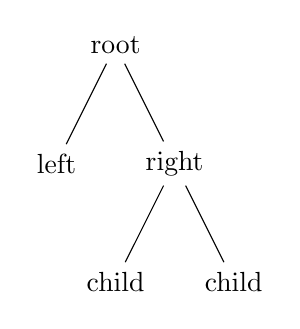
\begin{tikzpicture}
  \node {root}
    child {node {left}}
    child {node {right}
      child {node {child}}
      child {node {child}}
    };
\end{tikzpicture}
\end{codeexample}
%
% Since trees are made up from nodes, it is possible to use options to modify the way trees are drawn. Here are two examples of the above tree, redrawn with different options:
%
由于树是由节点组成的,所以可以使用选项来修改树的绘制方式。下面是上述树的两个例子,用不同的选项重新绘制:
%
\begin{codeexample}[preamble={\usetikzlibrary{arrows.meta,trees}}]
\begin{tikzpicture}
  [edge from parent fork down, sibling distance=15mm, level distance=15mm,
   every node/.style={fill=red!30,rounded corners},
   edge from parent/.style={red,-{Circle[open]},thick,draw}]
  \node {root}
      child {node {left}}
      child {node {right}
        child {node {child}}
        child {node {child}}
      };
\end{tikzpicture}
\end{codeexample}

\begin{codeexample}[]
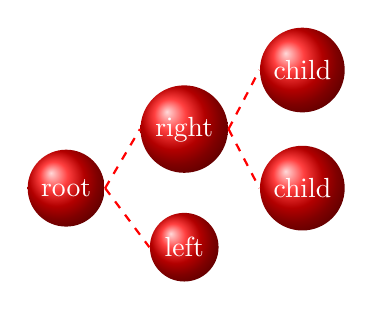
\begin{tikzpicture}
  [parent anchor=east,child anchor=west,grow=east,
   sibling distance=15mm, level distance=15mm,
   every node/.style={ball color=red,circle,text=white},
   edge from parent/.style={draw,dashed,thick,red}]
  \node {root}
      child {node {left}}
      child {node {right}
        child {node {child}}
        child {node {child}}
      };
\end{tikzpicture}
\end{codeexample}


% \subsection{Special Syntax for Graphs}
\subsection{用于指定 \texttt{graph} 的特殊语法}

% The |\node| command gives you fine control over where nodes should be placed, what text they should use, and what they should look like. However, when you draw a graph, you typically need to create numerous fairly similar nodes that only differ with respect to the name they show. In these cases, the |graph| syntax can be used, which is another syntax layer build ``on top'' of the node syntax.

|\node| 命令可以很好地控制节点应该放置在何处、节点应该使用什么文本以及节点的外观。但是,在绘制图形时,通常需要创建许多非常类似的节点,这些节点的不同之处在于它们所显示的名称。在这些情况下,可以使用 |graph| 语法,这是在节点语法之上构建的另一个语法层。
%
\begin{codeexample}[preamble={\usetikzlibrary{graphs}}]
\tikz \graph [grow down, branch right] {
  root -> { left, right -> {child, child} }
};
\end{codeexample}
%
% The syntax of the |graph| command extends the so-called \textsc{dot}-notation used in the popular \textsc{graphviz} program.
%
|\graph| 命令的语法扩展了流行的\textsc{graphviz}程序中使用的所谓的\textsc{dot}表示法。

% Depending on the version of \TeX\ you use (it must allow you to call Lua code, which is the case for Lua\TeX), you can also ask \tikzname\ to do automatically compute good positions for the nodes of a graph using one of several integrated \emph{graph drawing algorithms}.

根据您使用的\TeX\ 的版本(它必须允许您调用Lua代码,这是Lua\TeX 的情况),您还可以要求\tikzname\ 使用几种集成的\emph{图形绘制算法}之一来自动计算图形节点的良好位置。


% \subsection{Grouping of Graphic Parameters}
\subsection{图形参数的分组}

% Graphic parameters should often apply to several path drawing or filling commands. For example, we may wish to draw numerous lines all with the same line width of 1pt. For this, we put these commands in a |{scope}| environment that takes the desired graphic options as an optional parameter. Naturally, the specified graphic parameters apply only to the drawing and filling commands inside the environment. Furthermore, nested |{scope}| environments or individual drawing commands can override the graphic parameters of outer |{scope}| environments. In the following example, three red lines, two green lines, and one blue line are drawn:

图形参数应该经常应用于几个路径绘制或填充命令。例如,我们可能希望绘制多条线,所有线宽都为1pt。为此,我们将这些命令放在 |{scope}| 环境中,该环境将所需的图形选项作为可选参数。当然,指定的图形参数仅应用于环境中的绘图和填充命令。此外,嵌套 |{scope}| 环境或单个绘制命令可以覆盖外部 |{scope}| 环境的图形参数。在下面的例子中,画了三条红线,两条绿线,一条蓝线:
%
\begin{codeexample}[]
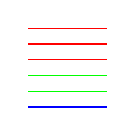
\begin{tikzpicture}
  \begin{scope}[color=red]
    \draw (0mm,10mm) -- (10mm,10mm);
    \draw (0mm, 8mm) -- (10mm, 8mm);
    \draw (0mm, 6mm) -- (10mm, 6mm);
  \end{scope}
  \begin{scope}[color=green]
    \draw             (0mm, 4mm) -- (10mm, 4mm);
    \draw             (0mm, 2mm) -- (10mm, 2mm);
    \draw[color=blue] (0mm, 0mm) -- (10mm, 0mm);
  \end{scope}
\end{tikzpicture}
\end{codeexample}

% The |{tikzpicture}| environment itself also behaves like a |{scope}| environment, that is, you can specify graphic parameters using an optional argument. These optional apply to all commands in the picture.

|{tikzpicture}| 环境本身的行为也类似于 |{scope}| 环境,也就是说,您可以使用可选参数指定图形参数。这些可选命令适用于图片中的所有命令。


% \subsection{Coordinate Transformation System}
\subsection{坐标转换系统}

% \tikzname\ supports both \pgfname's \emph{coordinate} transformation system to perform transformations as well as \emph{canvas} transformations, a more low-level transformation system. (For details on the difference between coordinate transformations and canvas transformations see Section~\ref{section-design-transformations}.)

\tikzname\ 同时支持\pgfname 的\emph{坐标}转换系统来执行转换,以及\emph{画布}转换,这是一种更低级的转换系统。(关于坐标转换和画布转换之间区别的详细信息,请参阅第\ref{section-design-transformations}节。)

% The syntax is set up in such a way that it is harder to use canvas transformations than coordinate transformations. There are two reasons for this: First, the canvas transformation must be used with great care and often results in ``bad'' graphics with changing line width and text in wrong sizes. Second, \pgfname\ loses track of where nodes and shapes are positioned when canvas transformations are used. So, in almost all circumstances, you should use coordinate transformations rather than canvas transformations.

语法的设置使得使用画布转换比使用坐标转换更困难。这样做有两个原因:首先,画布转换的使用必须非常小心,经常会导致``糟糕''的图形,改变了线宽和文本的大小。其次,当使用画布转换时,\pgfname\ 失去了对节点和形状位置的跟踪。因此,在几乎所有的情况下,您应该使用坐标转换而不是画布转换。

\clearpage
\input{parts/TikZ-ist-kein-Zeichenprogramm/sections/pgfmanual-zh-tikz-scopes}
% \input{parts/TikZ-ist-kein-Zeichenprogramm/sections/pgfmanual-zh-tikz-coordinates}
% \input{parts/TikZ-ist-kein-Zeichenprogramm/sections/pgfmanual-zh-tikz-paths}
% \input{parts/TikZ-ist-kein-Zeichenprogramm/sections/pgfmanual-zh-tikz-actions}
% \input{parts/TikZ-ist-kein-Zeichenprogramm/sections/pgfmanual-zh-tikz-arrows}
% \input{parts/TikZ-ist-kein-Zeichenprogramm/sections/pgfmanual-zh-tikz-shapes}
% \input{parts/TikZ-ist-kein-Zeichenprogramm/sections/pgfmanual-zh-tikz-pics}
% \input{parts/TikZ-ist-kein-Zeichenprogramm/sections/pgfmanual-zh-tikz-graphs}
% \input{parts/TikZ-ist-kein-Zeichenprogramm/sections/pgfmanual-zh-tikz-matrices}
% \input{parts/TikZ-ist-kein-Zeichenprogramm/sections/pgfmanual-zh-tikz-trees}
% \input{parts/TikZ-ist-kein-Zeichenprogramm/sections/pgfmanual-zh-tikz-plots}
% \input{parts/TikZ-ist-kein-Zeichenprogramm/sections/pgfmanual-zh-tikz-transparency}
% \input{parts/TikZ-ist-kein-Zeichenprogramm/sections/pgfmanual-zh-tikz-decorations}
% \input{parts/TikZ-ist-kein-Zeichenprogramm/sections/pgfmanual-zh-tikz-transformations}
% \input{parts/TikZ-ist-kein-Zeichenprogramm/sections/pgfmanual-zh-tikz-animations}
% \part{Graph Drawing}
\label{part-gd}

{\Large \emph{by Till Tantau et al.}}

\bigskip
\noindent
\emph{Graph drawing algorithms} do the tough work of computing a layout of a
graph for you. \tikzname\ comes with powerful such algorithms, but you can also
implement new algorithms in the Lua programming language. \vskip1cm

\ifluatex
\begin{codeexample}[
    graphic=white,
    preamble={\usetikzlibrary{arrows.meta,graphs,graphdrawing}
\usegdlibrary{layered}}]
\tikz [nodes={text height=.7em, text depth=.2em,
              draw=black!20, thick, fill=white, font=\footnotesize},
       >={Stealth[round,sep]}, rounded corners, semithick]
  \graph [layered layout, level distance=1cm, sibling sep=.5em, sibling distance=1cm] {
    "5th Edition" -> { "6th Edition", "PWB 1.0" };
    "6th Edition" -> { "LSX" [>child anchor=45],  "1 BSD", "Mini Unix", "Wollongong", "Interdata" };
    "Interdata" -> { "Unix/TS 3.0", "PWB 2.0", "7th Edition" };
    "7th Edition" -> { "8th Edition", "32V", "V7M", "Ultrix-11", "Xenix", "UniPlus+" };
    "V7M" -> "Ultrix-11";
    "8th Edition" -> "9th Edition";
    "1 BSD" -> "2 BSD" -> "2.8 BSD" -> { "Ultrix-11", "2.9 BSD" };
    "32V" -> "3 BSD" -> "4 BSD" -> "4.1 BSD" -> { "4.2 BSD", "2.8 BSD", "8th Edition" };
    "4.2 BSD" -> { "4.3 BSD", "Ultrix-32" };
    "PWB 1.0" -> { "PWB 1.2" -> "PWB 2.0", "USG 1.0" -> { "CB Unix 1", "USG 2.0" }};
    "CB Unix 1" -> "CB Unix 2" -> "CB Unix 3" -> { "Unix/TS++", "PDP-11 Sys V" };
    { "USG 2.0" -> "USG 3.0", "PWB 2.0", "Unix/TS 1.0" } -> "Unix/TS 3.0";
    { "Unix/TS++", "CB Unix 3", "Unix/TS 3.0" } -> "TS 4.0" -> "System V.0" -> "System V.2" -> "System V.3";
  };
\end{codeexample}

\else
    You need to use Lua\TeX\ to typeset this part of the manual (and, also, to
    use algorithmic graph drawing).
\fi

\input{parts/Graph-Drawing/sections/pgfmanual-zh-gd-overview}
\input{parts/Graph-Drawing/sections/pgfmanual-zh-gd-usage-tikz}
\input{parts/Graph-Drawing/sections/pgfmanual-zh-gd-usage-pgf}
\input{parts/Graph-Drawing/sections/pgfmanual-zh-gd-trees}
\input{parts/Graph-Drawing/sections/pgfmanual-zh-gd-layered}
\input{parts/Graph-Drawing/sections/pgfmanual-zh-gd-force}
\input{parts/Graph-Drawing/sections/pgfmanual-zh-gd-circular}
\input{parts/Graph-Drawing/sections/pgfmanual-zh-gd-phylogenetics}
\input{parts/Graph-Drawing/sections/pgfmanual-zh-gd-edge-routing}
%
% XXX : disabled because of
% 1. compile-time dependencies which are hard to resolve
% 2. it is "hardly usable anyway" (TT)
%\input{parts/Graph-Drawing/sections/pgfmanual-zh-gd-ogdf}
\input{parts/Graph-Drawing/sections/pgfmanual-zh-gd-algorithm-layer}
\input{parts/Graph-Drawing/sections/pgfmanual-zh-gd-algorithms-in-c}
\input{parts/Graph-Drawing/sections/pgfmanual-zh-gd-display-layer}
\input{parts/Graph-Drawing/sections/pgfmanual-zh-gd-binding-layer}
% \part{Libraries}
\label{part-libraries}

{\Large \emph{by Till Tantau}}


\bigskip
\noindent
In this part the library packages are documented. They provide additional
predefined graphic objects like new arrow heads or new plot marks, but
sometimes also extensions of the basic \pgfname\ or \tikzname\ system. The
libraries are not loaded by default since many users will not need them.

\medskip
\noindent
\begin{codeexample}[graphic=white,preamble={\usetikzlibrary{arrows,trees}}]
\tikzset{
  ld/.style={level distance=#1},lw/.style={line width=#1},
  level 1/.style={ld=4.5mm, trunk,          lw=1ex ,sibling angle=60},
  level 2/.style={ld=3.5mm, trunk!80!leaf a,lw=.8ex,sibling angle=56},
  level 3/.style={ld=2.75mm,trunk!60!leaf a,lw=.6ex,sibling angle=52},
  level 4/.style={ld=2mm,   trunk!40!leaf a,lw=.4ex,sibling angle=48},
  level 5/.style={ld=1mm,   trunk!20!leaf a,lw=.3ex,sibling angle=44},
  level 6/.style={ld=1.75mm,leaf a,         lw=.2ex,sibling angle=40},
}
\pgfarrowsdeclare{leaf}{leaf}
  {\pgfarrowsleftextend{-2pt} \pgfarrowsrightextend{1pt}}
{
  \pgfpathmoveto{\pgfpoint{-2pt}{0pt}}
  \pgfpatharc{150}{30}{1.8pt}
  \pgfpatharc{-30}{-150}{1.8pt}
  \pgfusepathqfill
}

\newcommand{\logo}[5]
{
  \colorlet{border}{#1}
  \colorlet{trunk}{#2}
  \colorlet{leaf a}{#3}
  \colorlet{leaf b}{#4}
  \begin{tikzpicture}
    \scriptsize\scshape
    \draw[border,line width=1ex,yshift=.3cm,
          yscale=1.45,xscale=1.05,looseness=1.42]
      (1,0) to [out=90, in=0]    (0,1)  to [out=180,in=90]  (-1,0)
            to [out=-90,in=-180] (0,-1) to [out=0,  in=-90] (1,0) -- cycle;

    \coordinate (root) [grow cyclic,rotate=90]
    child {
      child [line cap=round] foreach \a in {0,1} {
        child foreach \b in {0,1} {
          child foreach \c in {0,1} {
            child foreach \d in {0,1} {
              child foreach \leafcolor in {leaf a,leaf b}
                { edge from parent [color=\leafcolor,-#5] }
        } } }
      } edge from parent [shorten >=-1pt,serif cm-,line cap=butt]
    };

    \node [align=center,below] at (0pt,-.5ex)
    { \textcolor{border}{T}heoretical \\ \textcolor{border}{C}omputer \\
      \textcolor{border}{S}cience };
  \end{tikzpicture}
}
\begin{minipage}{3cm}
  \logo{green!80!black}{green!25!black}{green}{green!80}{leaf}\\
  \logo{green!50!black}{black}{green!80!black}{red!80!green}{leaf}\\
  \logo{red!75!black}{red!25!black}{red!75!black}{orange}{leaf}\\
  \logo{black!50}{black}{black!50}{black!25}{}
\end{minipage}
\end{codeexample}

\input{parts/Libraries/sections/pgfmanual-zh-library-3d}
\input{parts/Libraries/sections/pgfmanual-zh-library-angles}
\input{parts/Libraries/sections/pgfmanual-zh-library-arrows}
\input{parts/Libraries/sections/pgfmanual-zh-library-automata}
\input{parts/Libraries/sections/pgfmanual-zh-library-babel}
\input{parts/Libraries/sections/pgfmanual-zh-library-backgrounds}
\input{parts/Libraries/sections/pgfmanual-zh-library-bbox}
\input{parts/Libraries/sections/pgfmanual-zh-library-calc}
\input{parts/Libraries/sections/pgfmanual-zh-library-calendar}
\input{parts/Libraries/sections/pgfmanual-zh-library-chains}
\input{parts/Libraries/sections/pgfmanual-zh-library-circuits}
\input{parts/Libraries/sections/pgfmanual-zh-library-decorations}
\input{parts/Libraries/sections/pgfmanual-zh-library-er}
\input{parts/Libraries/sections/pgfmanual-zh-library-external}
\input{parts/Libraries/sections/pgfmanual-zh-library-fadings}
\input{parts/Libraries/sections/pgfmanual-zh-library-fit}
\input{parts/Libraries/sections/pgfmanual-zh-library-fixedpoint}
\input{parts/Libraries/sections/pgfmanual-zh-library-fpu}
\input{parts/Libraries/sections/pgfmanual-zh-library-lsystems}
\input{parts/Libraries/sections/pgfmanual-zh-library-math}
\input{parts/Libraries/sections/pgfmanual-zh-library-matrices}
% Copyright 2019 by Till Tantau
%
% This file may be distributed and/or modified
%
% 1. under the LaTeX Project Public License and/or
% 2. under the GNU Free Documentation License.
%
% See the file doc/generic/pgf/licenses/LICENSE for more details.


% \section{Mindmap Drawing Library}
\section{思维导图图形库}

\begin{tikzlibrary}{mindmap}
   % This packages provides styles for drawing mindmap diagrams.

    该包提供了用于绘制思维导图的样式。
\end{tikzlibrary}

% \subsection{Overview}
\subsection{概述}

% This library is intended to make the creation of mindmaps or concept maps easier. A \emph{mindmap} is a graphical representation of a concept together with related concepts and annotations. Mindmaps are, essentially, trees, possibly with a few extra edges added, but they are usually drawn in a special way: The root concept is placed in the middle of the page and is drawn as a huge circle, ellipse, or cloud. The related concepts then ``leave'' this root concept via branch-like tendrils.

该库旨在简化思维导图或概念图的创建。 \emph{思维导图} 是一个用于表示概念和相关概念以及注释的图形。 思维导图本质上是树,可能添加了一些额外的边,但通常以特殊的方式绘制:根概念位于页面的中间,并绘制为巨大的圆形,椭圆形或云形。 然后,相关的概念通过类似树枝的卷须``离开''这个根概念。

% The |mindmap| library of \tikzname\ produces mindmaps that look a bit different from the standard mindmaps: While the big root concept is still a circle, related concepts are also depicted as (smaller) circles. The related concepts are linked to the root concept via organic-looking connections. The overall effect is visually rather pleasing, but readers may not immediately think of a mindmap when they see a picture created with this library.

由\tikzname 的 |mindmap| 库绘制的思维导图看起来与标准思维导图有些不同:虽然大根概念仍然是一个圆,相关概念也被描述为(较小)圆。 相关概念通过外观相似的连接链接到根概念。 总体效果在视觉上令人愉悦,但是当读者看到使用此库创建的图片时,可能不会立即想到思维导图。

% Although it is not strictly necessary, you will usually create mindmaps using \tikzname's tree mechanism and some of the styles and macros of the package work best when used inside trees. However, it is still possible and sometimes necessary to treat parts of a mindmap as a graph with arbitrary edges and this is also possible.

尽管不是绝对必要的,但是通常您会使用\tikzname 的树机制来创建思维导图,并且在树内使用时,包的某些样式和宏效果最佳。 但是,仍然可能并且有时有必要将思维导图的各个部分视为具有任意边的图,这也是可能的。


% \subsection{The Mindmap Style}
\subsection{思维导图样式}

% Every mindmap should be put in a scope or a picture where the |mindmap| style is used. This style installs some internal settings.

每个思维导图都应放在使用 |mindmap| 样式的作用域或图片环境中。 此样式将加载一些内部设置。

\begin{stylekey}{/tikz/mindmap}
    % Use this style with all pictures or at least scopes that contain a mindmap. It installs a whole bunch of settings that are useful for drawing mindmaps.

    对所有图片或至少包含思维导图的图片使用这种风格。它安装了一大堆对绘制思维导图有用的设置。
    %
\begin{codeexample}[preamble={\usetikzlibrary{mindmap}}]
\tikz[mindmap,concept color=red!50]
  \node [concept] {Root concept}
    child[grow=right] {node[concept] {Child concept}};
\end{codeexample}
    %
    %The sizes of concepts are predefined in such a way that a medium-size mindmap will fit on an A4 page (more or less).
    
    预定义概念的大小,以使中型思维导图适合A4页面(或多或少)。
    %
    \begin{stylekey}{/tikz/every mindmap}
        % This style is included by the |mindmap| style. Change this style to add special settings to your mindmaps.

        这种样式包含在 |mindmap| 样式中。改变这种样式,为你的思维导图添加特殊设置。
        %
\begin{codeexample}[preamble={\usetikzlibrary{mindmap}}]
\tikz[large mindmap,concept color=red!50]
  \node [concept] {Root concept}
    child[grow=right] {node[concept] {Child concept}};
\end{codeexample}
    \end{stylekey}

    % \paragraph{Remark:}
    % Note that |mindmap| redefines |font| sizes and |sibling angle| depending on the current concept level (i.e. inside of |level 1 concept|, |level 2 concept| etc.). Thus, if you need to redefine these variables, use

    \paragraph{备注}
    注意 |mindmap| 重新定义 |font| 大小和 |sibling angle|,取决于当前概念级别(即 |level 1 concept|,|level 2 concept| 等中的概念)。 因此,如果您需要重新定义这些变量,请使用

    |level 1 concept/.append style={font=\small}|

    % \noindent or
    \noindent 或

    |level 2 concept/.append style={sibling distance=90}|

    % \noindent \emph{after} the |mindmap| style.

    应在 |mindmap| 样式\emph{之后}使用。
\end{stylekey}

\begin{stylekey}{/tikz/small mindmap}
    % This style includes the |mindmap| style, but additionally changes the
    default size of concepts, fonts and distances so that a medium-sized
    mindmap will fit on an A5 page (A5 pages are half as large as A4 pages). Mindmaps with |small mindmap| will also fit onto a standard frame of the |beamer| package.

    此样式包含 |mindmap| 样式,但另外会更改概念,字体和距离的默认大小,以使中型思维导图适合A5页面(A5页面的大小是A4页面的一半)。 具有 |small mindmap| 的思维导图适合| beamer | 宏包的标准框架。
\end{stylekey}

\begin{stylekey}{/tikz/large mindmap}
    % This style includes the |mindmap| style, but additionally changes the default size of concepts, fonts and distances so that a medium-sized mindmap will fit on an A3 page (A3 pages are twice as large as A4 pages).

    此样式包含 |mindmap| 样式,但另外会更改概念,字体和距离的默认大小,以使中型思维导图适合A3页面(A3页面的大小是A4页面的两倍)。
\end{stylekey}

\begin{stylekey}{/tikz/huge mindmap}
    % This style causes concepts to be even bigger and it is best used with A2 paper and above.

    这种样式会使概念更大,最好与A2纸及更高版本一起使用。
\end{stylekey}


% \subsection{Concepts Nodes}
\subsection{概念节点}

% The basic entities of mindmaps are called \emph{concepts} in \tikzname. A concept is a node of style |concept| and it must be circular for some of the connection macros to work.

思维导图的基本实体在\tikzname 中被称为\emph{概念}。 概念是样式为 |concept| 的节点,它必须是圆形的,这样一些连接宏才能正常工作。

% \subsubsection{Isolated Concepts}
\subsubsection{孤立的概念}

% The following styles influence how isolated concepts are rendered:

以下样式影响孤立概念的呈现方式:

\begin{stylekey}{/tikz/concept}
    % This style should be used with all nodes that are concepts, although some styles like |extra concept| install this style automatically.

    尽管某些样式(如 |extra concept|)自动加载此样式,该样式应与所有作为概念的节点一起使用。

    % Basically, this style makes the concept node circular and installs a uniform color called |concept color|, see below. Additionally, the style |every concept| is called.

    基本上,这种样式使概念节点成为圆形,并加载被称为 |concept color| 的统一颜色,请参见下文。 此外,样式 |every concept| 被自动加载。
    %
\begin{codeexample}[preamble={\usetikzlibrary{mindmap}}]
\tikz[mindmap,concept color=red!50] \node [concept] {Some concept};
\end{codeexample}

    \begin{stylekey}{/tikz/every concept}
        % In order to change the appearance of concept nodes, you should change this style. Note, however, that the color of a concept should be uniform for some of the connection bar stuff to work, so you should not change the color or the draw/fill state of concepts using this option. It is mostly useful for changing the text color and font.

        为了更改概念节点的外观,您应该更改此样式。 但是请注意,对于某些连接带来说,概念的颜色应该统一,因此您不应使用此选项更改概念的颜色或绘制/填充状态。 它对于更改文本颜色和字体很有用。
    \end{stylekey}

    \begin{key}{/tikz/concept color=\meta{color}}
        % This option tells \tikzname\ which color should be used for filling and stroking concepts. The difference between this option and just setting |every concept| to the desired color is that this option allows \tikzname\ to keep track of the colors used for concepts. This is important when you \emph{change} the color between two connected concepts. In this case, \tikzname\ can automatically create a shading that provides a smooth transition between the old and the new concept color; we will come back to this in the next section.

        这个选项告诉\tikzname\ 哪种颜色应该用于填充和描边概念。此选项与直接将 |every concept| 设置为所需颜色的区别在于,此选项允许\tikzname\ 跟踪用于概念的颜色。当你在两个相连的概念之间改变颜色时,这一点很重要。在这种情况下,\tikzname\ 可以自动创建阴影,提供新旧概念颜色之间的平滑过渡;我们将在下一节中回到这个问题。
    \end{key}
\end{stylekey}

\begin{stylekey}{/tikz/extra concept}
    % This style is intended for concepts that are not part of the ``mindmap tree'', but stand beside it. Typically, they will have a subdued color or be smaller. In order to have these concepts appear in a uniform way and in order to indicate in the code that these concepts are additional, you can use this style.

    此样式适用于不属于``思维导图''但位于其旁边的概念。 通常,它们将具有更淡的颜色或更小的尺寸。 为了绘制这些概念并在代码中指出这些概念是附加的,可以使用此样式。
    %
\begin{codeexample}[preamble={\usetikzlibrary{mindmap}}]
\begin{tikzpicture}[mindmap,concept color=blue!80]
  \node [concept]                 {Root concept};
  \node [extra concept] at (10,0) {extra concept};
\end{tikzpicture}
\end{codeexample}
    %
    \begin{stylekey}{/tikz/every extra concept}
        % Change this style to change the appearance of extra concepts.

        更改此样式可更改其他概念的外观。
    \end{stylekey}
\end{stylekey}


% \subsubsection{Concepts in Trees}
\subsubsection{树中的概念}

% As pointed out earlier, \tikzname\ assumes that your mindmap is built using the |child| facilities of \tikzname. There are numerous options that influence how concepts are rendered at the different levels of a tree.

正如前面指出的,\tikzname\ 假设您的思维导图是使用 \tikzname 的 |child| 工具构建的。有许多选项影响如何在树的不同级别上呈现概念。

\begin{stylekey}{/tikz/root concept}
    % This style is used for the roots of mindmap trees. By adding something to this, you can change how the root of a mindmap will be rendered.

    此样式用于思维导图树的根节点。 通过添加一些东西,您可以更改思维导图的根节点的渲染方式。
    %
\begin{codeexample}[preamble={\usetikzlibrary{mindmap}}]
\tikz
  [root concept/.append style={concept color=blue!80,minimum size=3.5cm},
   mindmap]
  \node [concept] {Root concept};
\end{codeexample}

    % Note that styles like |large mindmap| redefine these styles, so you should add something to this style only inside the picture.

    请注意 |large mindmap| 重新定义这些样式,因此您应该仅在图片内向此样式添加一些内容。
\end{stylekey}

\begin{stylekey}{/tikz/level 1 concept}
    % The |mindmap| style adds this style to the |level 1| style. This means that the first level children of a mindmap tree will use this style.

    |mindmap| 样式将此样式添加到 |level 1| 样式,这意味着思维导图树的第一级子代将使用此样式。
    %
\begin{codeexample}[preamble={\usetikzlibrary{mindmap}}]
\tikz
  [root concept/.append style={concept color=blue!80},
   level 1 concept/.append style={concept color=red!50},
   mindmap]
  \node [concept] {Root concept}
    child[grow=30] {node[concept] {child}}
    child[grow=0 ] {node[concept] {child}};
\end{codeexample}
\end{stylekey}

\begin{stylekey}{/tikz/level 2 concept}
    % Works like |level 1 concept|, only for second level children.

    类似于 |level 1 concept|,仅适用于第二级子代。
\end{stylekey}

\begin{stylekey}{/tikz/level 3 concept}
    % Works like |level 1 concept|.

    类似于 |level 1 concept|。
\end{stylekey}

\begin{stylekey}{/tikz/level 4 concept}
    % Works like |level 1 concept|. Note that there are no fifth and higher level styles, you need to modify |level 5| directly in such cases.

    类似于 |level 1 concept|。注意,没有第五种和更高级别的样式,在这种情况下您需要直接修改 |level 5|。
\end{stylekey}

\begin{key}{/tikz/concept color=\meta{color}}
    % We saw already that this option is used to change the color of concepts. We now have a look at its effect when used on child nodes of a concept. Normally, this option simply changes the color of the children. However, when the option is given as an option to the |child| operation (and not to the |node| operation and also not as an option to all children via the |level 1| style), \tikzname\ will smoothly change the concept color from the parent's color to the color of the child concept.

    我们已经看到该选项用于更改概念的颜色。 现在我们来看看它在概念的子节点上使用时的效果。 通常,此选项仅更改子项的颜色。 但是,当将该选项作为 |child| 操作的选项(而不是对 |node| 操作的选项,也不是通过 |level 1| 样式给所有子级提供的选项),\tikzname\ 将平滑地将概念颜色从父级概念颜色过渡为子级概念的颜色。

    % Here is an example:

    这是一个例子:
    %
\begin{codeexample}[preamble={\usetikzlibrary{mindmap}}]
\tikz[mindmap,concept color=blue!80]
  \node [concept] {Root concept}
    child[concept color=red,grow=30] {node[concept] {Child concept}}
    child[concept color=orange,grow=0]  {node[concept] {Child concept}};
\end{codeexample}

    % In order to have a concept color which changes with the hierarchy level, a tiny bit of magic is needed:

    为了使概念颜色随层次结构级别而变化,需要一点魔法:

% FIXME: is this a bug in the software!? The root concept is black!?
\begin{codeexample}[preamble={\usetikzlibrary{mindmap}}]
\tikz[mindmap,text=white,
      root concept/.style={concept color=blue},
      level 1 concept/.append style=
        {every child/.style={concept color=blue!50}}]
  \node [concept] {Root concept}
    child[grow=30] {node[concept] {child}}
    child[grow=0 ] {node[concept] {child}};
\end{codeexample}
    %
\end{key}


% \subsection{Connecting Concepts}
\subsection{连接概念}

% \subsubsection{Simple Connections}
\subsubsection{简单连接}

% The easiest way to connect two concepts is to draw a line between them. In order to give such lines a consistent appearance, it is recommendable to use the following style when drawing such lines:

连接两个概念的最简单方法是在它们之间画一条线。 为了使此类线条具有一致的外观,建议在绘制此类线条时使用以下样式:

\begin{stylekey}{/tikz/concept connection}
    % This style can be used for lines between two concepts. Feel free to redefine this style.

    此样式可用于两个概念之间的线条。可随意重新定义此样式。
\end{stylekey}

% A problem arises when you need to connect concepts after the main mindmap has been drawn. In this case you will want the connection lines to lie \emph{behind} the main mindmap. However, you can draw the lines only after the coordinates of the concepts have been determined. In this case you should place the connecting lines on a background layer as in the following example:

在绘制主思维导图之后需要连接概念时,会出现问题。 在这种情况下,您将希望连接线位于主思维导图的\emph{后面}。 但是,仅在确定概念的坐标之后才能绘制线。 在这种情况下,应将连接线放在背景层上,如以下示例所示:

\begin{codeexample}[preamble={\usetikzlibrary{backgrounds,mindmap}}]
\begin{tikzpicture}
  [root concept/.append style={concept color=blue!20,minimum size=2cm},
   level 1 concept/.append style={sibling angle=45},
   mindmap]
  \node [concept] {Root concept}
    [clockwise from=45]
    child { node[concept] (c1) {child}}
    child { node[concept] (c2) {child}}
    child { node[concept] (c3) {child}};
  \begin{pgfonlayer}{background}
    \draw [concept connection]  (c1) edge (c2)
                                     edge (c3)
                                (c2) edge (c3);
  \end{pgfonlayer}
\end{tikzpicture}
\end{codeexample}


% \subsubsection{The Circle Connection Bar Decoration}
\subsubsection{圆形带连接}

% Instead of a simple line between two concepts, you can also add a bar between the two nodes that has slightly organic ends. These bars are also used by default as the edges from parents in the mindmap tree.

除了在两个概念之间创建简单的线条外,您还可以在两个节点之间添加一条稍微带有一点有机末端的带状图。 默认情况下,这些带也用作思维导图树中父级概念的边。

% For the drawing of the bars a special decoration is used, which is defined in the |mindmap| library:

对于带的绘制,使用了特殊的修饰,该修饰在 |mindmap| 库中定义:

\begin{decoration}{circle connection bar}
    % This decoration can be used to connect two circles. The start of the
    to-be-decorated path should lie on the border of the first circle, the end should lie on the border of the second circle. The following two decoration keys should be initialized with the sizes of the circles:

    此修饰可用于连接两个圆。 待修饰路径的起点应在第一个圆的边界上,终点应在第二个圆的边界上。 以下两个修饰键应使用圆的大小初始化:
    %
    \begin{itemize}
        \item |start radius|
        \item |end radius|
    \end{itemize}
    %
    % Furthermore, the following two decoration keys influence the decoration:
    % 
    此外,以下两个修饰键会影响修饰:
    %
    \begin{itemize}
        \item |amplitude|
        \item |angle|
    \end{itemize}
    %
    % The decoration turns a straight line into a path that starts on the border of the first circle at the specified angle relative to the line connecting the centers of the circles. The path then changes into a rectangle whose thickness is given by the amplitude. Finally, the path ends with the same angles on the second circle.

    该修饰将直线转变为路径,该路径从第一个圆的边界开始,相对于连接圆的圆心的线的指定角度。然后,路径变成一个矩形,其厚度由幅度给定。最后,路径以第二个圆上相同的角度结束。

    % Here is an example that should make this clearer:

    这是一个应该更清楚地说明示例:
    %
\begin{codeexample}[preamble={\usetikzlibrary{mindmap}}]
\begin{tikzpicture}
    [decoration={start radius=1cm,end radius=.5cm,amplitude=2mm,angle=30}]
  \fill[blue!20] (0,0)   circle (1cm);
  \fill[red!20]  (2.5,0) circle (.5cm);

  \filldraw [draw=red,fill=black,
             decorate,decoration=circle connection bar] (1,0) -- (2,0);
\end{tikzpicture}
\end{codeexample}

    % As can be seen, the decorated path consists of three parts and is not really useful for drawing. However, if you fill the decorated path only, and if you use the same color as for the circles, the result is better.

    可以看出,修饰的路径由三部分组成,对于绘图并没有真正的用处。 但是,如果仅填充修饰的路径,并且使用与圆相同的颜色,则效果会更好。
    %
\begin{codeexample}[preamble={\usetikzlibrary{mindmap}}]
\begin{tikzpicture}
  [blue!50,decoration={start radius=1cm,
                       end radius=.5cm,amplitude=2mm,angle=30}]
  \fill (0,0)   circle (1cm);
  \fill (2.5,0) circle (.5cm);

  \fill [decorate,decoration=circle connection bar] (1,0) -- (2,0);
\end{tikzpicture}
\end{codeexample}

    % In the above example you may notice the small white line between the circles and the decorated path. This is due to rounding errors. Unfortunately, for larger distances, the errors can accumulate quite strongly, especially since \tikzname\ and \TeX\ are not very good at computing square roots. For this reason, it is a good idea to make the circles slightly larger to cover up such problems. When using nodes of shape |circle|, you can just add the |draw| option with a |line width| of one or two points (for very large distances you may need line width up to 4pt).

    在上面的示例中,您可能会注意到圆和修饰路径之间的白色小线。 这是由于舍入误差造成的。 不幸的是,对于更大的距离,错误会累积得非常强烈,特别是因为\tikzname\ 和\TeX\ 不太善于计算平方根。 因此,最好使圆稍大一些以掩盖此类问题。 当使用形状为 |circ| 的节点时,只需添加 |draw| 的 |line width| 的选项增加1pt或2pt(对于非常长的距离,您可能需要最大4pt的线宽)。
    %
\begin{codeexample}[preamble={\usetikzlibrary{mindmap}}]
\begin{tikzpicture}
  [blue!50,decoration={start radius=1cm,
                       end radius=.5cm,amplitude=2mm,angle=30}]
  \fill (0,0)   circle (1cm+1pt);
  \fill (2.4,0) circle (.5cm+1pt);

  \fill [decorate,decoration=circle connection bar] (1,0) -- (1.9,0);
\end{tikzpicture}
\end{codeexample}

    % FIXME: this paragraph appears to be deprecated:
    %Note the slightly strange |outer sep=0pt|. This is needed so that
    %the decorated path lies on the border of the filled circle, not on the
    %border of the stroked circle (which is slightly larger and this
    %slightly larger size is exactly what we wish to use to cover up the
    %rounding errors).
\end{decoration}


% \subsubsection{The Circle Connection Bar To-Path}
\subsubsection{圆形连接带的To-Path}

% The |circle connection bar| decoration is a bit complicated to use. Especially specifying the radii is quite bothersome (the amplitude and the angle can be set once and for all). For this reason, the |mindmap| library defines a special to-path that performs the necessary computations for you.

|circle connection bar| 修饰使用起来有点复杂。 特别是指定半径非常麻烦(可以一劳永逸地设置幅度和角度)。因此, |mindmap| 库定义了一个特殊的to-path,可以为您执行必要的计算。

\begin{stylekey}{/tikz/circle connection bar}
    % This style installs a rather involved to-path. Unlike normal to-paths, this path requires that the start and the target of the to-path are named nodes of shape |circle| -- if this is not the case, this path will produce errors.

    这种样式会加载相当复杂的to-path。 与正常的to-path不同,此路径要求to-path的起点和目标为被其形状命名为 |circle| 的节点。 如果不是这种情况,该路径将产生错误。

    % Assuming that the start and the target are circles, the to-path will first compute the radii of these circles (by measuring the distance from the |center| anchor to some anchor on the border) and will set the |start circle| keys accordingly. Next, the |fill| option is set to the |concept color| while |draw=none| is set. The decoration is set to |circle connection bar|. Finally, the following style is included:

    假设起点和目标是圆,则to-path将首先计算这些圆的半径(通过测量从 |center| 锚点到边界上某个锚点的距离)并设置 |start circle| 键。 接下来,及时当 |draw=none| 选项被设置时 |fill| 选项也被设置为 |concept color|。 修饰设置为 |circle connection bar|。 最后,该样式包含以下样式:

    %
    \begin{stylekey}{/tikz/every circle connection bar}
        % Redefine this style to change the appearance of circle connection bar to-paths.

        重新定义此样式将改变圆形连接带路径的to-path。
    \end{stylekey}
    %
\begin{codeexample}[preamble={\usetikzlibrary{mindmap}}]
\begin{tikzpicture}[concept color=blue!50,blue!50,outer sep=0pt]
  \node (n1) at (0,0)   [circle,minimum size=2cm,fill,draw,thick] {};
  \node (n2) at (2.5,0) [circle,minimum size=1cm,fill,draw,thick] {};

  \path (n1) to[circle connection bar] (n2);
\end{tikzpicture}
\end{codeexample}
    %
    % Note that it is not a good idea to have more than one |to| operation together with the option |circle connection bar| in a single |\path|. Use the |edge| operation, instead, for creating multiple connections and this operation creates a new scope for each edge.

    注意,在一个 |\path| 中同时使用多个 |to| 操作和 |circle connection bar| 选项不是一个好主意。相反,使用 |edge| 操作创建多个连接,该操作为每条边创建一个新的范围。
\end{stylekey}

% In a mindmap we sometimes want colors to change from one concept color to another. Then, the connection bar should, ideally, consist of a smooth transition between these two colors. Getting this right using shadings is a bit tricky if you try this ``by hand'', so the  |mindmap| library provides a special option for facilitating this procedure.

在思维导图中,有时我们希望概念的颜色从一种颜色变为另一种。 然后,理想情况下,连接带应由这两种颜色之间的平滑过渡组成。 如果您``手工''尝试使用阴影完成这项工作,会有些棘手,因此 |mindmap| 库提供了一个特殊的选项来简化此过程。

\begin{key}{/tikz/circle connection bar switch color=|from (|\meta{first color}|) to (|\meta{second color}|)|} 
    % This style works similarly to the |circle connection bar|. The only difference is that instead of filling the path with a single color a shading is used.

    此样式的作用类似于 |circle connection bar|。 唯一的区别是,它不是使用单色填充路径,而是使用阴影。
    %
\begin{codeexample}[preamble={\usetikzlibrary{mindmap}}]
\begin{tikzpicture}[outer sep=0pt]
  \node (n1) at (0,0)    [circle,minimum size=2cm,fill,draw,thick,red] {};
  \node (n2) at (30:2.5) [circle,minimum size=1cm,fill,draw,thick,blue] {};

  \path (n1) to[circle connection bar switch color=from (red) to (blue)] (n2);
\end{tikzpicture}
\end{codeexample}
    %
\end{key}


% \subsubsection{Tree Edges}
\subsubsection{树的边}

% Most of the time, concepts in a mindmap are connected automatically when the mindmap is built as a tree. The reason is that the |mindmap| installs a |circle connection bar| path as the |edge from parent path|. Also, the |mindmap| option takes care of things like setting the correct |draw| and |outer sep| settings and some other stuff.

在大多数情况下,将思维导图构建为树时,思维导图中的概念会自动连接。 原因是 |mindmap| 加载了一个 |circle connection bar| 路径作为 |edge from parent path| 。 另外,|mindmap| 选项还可以处理诸如设置正确的 |draw| 和 |outer sep| 设置之类的事情。

% In detail, the |mindmap| option sets the |edge from parent path| to a path that uses the to-path |circle connection bar| to connect the parent node and the child node. The |concept color| option (locally) changes this by using |circle connection bar switch color| instead with the from-color set to the old (parent's) concept color and the to-color set to the new (child's) concept color. This means that when you provide the |concept color| option to a |child| command, the color will change from the parent's concept color to the specified color.

详细地说,|mindmap| 选项将 |edge from parent path| 设置为使用to-path |circle connection bar| 连接父节点和子节点的路径。|concept color| 选项(本地)通过使用 |circle connection bar switch color| 来改变这一点,而不是使用从颜色设置为旧的(父节点的)概念颜色和到颜色设置为新的(子节点的)概念颜色。这意味着,当您向一个 |child| 命令提供 |concept color| 选项时,颜色将从父节点概念颜色更改为指定的颜色。

% Let us now build a tree that way. Please note that we pass the |concept color| to the respective |child| and not to a |node| under it.

现在让我们用这种方法来构建一棵树。请注意,我们将 |concept color| 传递给相应的 |child|,而不是它下面的 |node|。
%
\begin{codeexample}[preamble={\usetikzlibrary{mindmap}}]
\begin{tikzpicture}
  \path[mindmap,concept color=black,text=white]
    node[concept] {Computer Science}
    [clockwise from=0]
    % note that `sibling angle' can only be defined in
    % `level 1 concept/.append style={}'
    child[concept color=green!50!black] {
      node[concept] {practical}
      [clockwise from=90]
      child { node[concept] {algorithms} }
      child { node[concept] {data structures} }
      child { node[concept] {pro\-gramming languages} }
      child { node[concept] {software engineer\-ing} }
    }
    % note that the `concept color' is passed to the `child'(!)
    child[concept color=blue] {
      node[concept] {applied}
      [clockwise from=-30]
      child { node[concept] {databases} }
      child { node[concept] {WWW} }
    }
    child[concept color=red] { node[concept] {technical} }
    child[concept color=orange] { node[concept] {theoretical} };
\end{tikzpicture}
\end{codeexample}


% \subsection{Adding Annotations}
\subsection{添加注释}

% An \emph{annotation} is some text outside a mindmap that, unlike an extra concept, simply explains something in the mindmap. The following style is mainly intended to help readers of the code see that a node in an annotation node.

\emph{注释}是思维导图之外的一些文本,与其他概念不同,它只是解释了思维导图中的某些内容。 下面的样式主要用于帮助代码的读者查看注释节点中的节点。

\begin{stylekey}{/tikz/annotation}
    % This style indicates that a node is an annotation node. It includes the style |every annotation|, which allows you to change this style in a convenient fashion.

    此样式表示节点是注释节点。 它包含 |every annotation| 样式,这使您可以方便地更改此样式。
    %
\begin{codeexample}[preamble={\usetikzlibrary{mindmap}}]
\begin{tikzpicture}
  [mindmap,concept color=blue!80,
  every annotation/.style={fill=red!20}]
  \node [concept] (root)  {Root concept};

  \node [annotation,right] at (root.east)
  {The root concept is, in general, the most important concept.};
\end{tikzpicture}
\end{codeexample}
    %
    \begin{stylekey}{/tikz/every annotation}
        %This style is included by |annotation|.

        此样式被 |annotation| 包含。
    \end{stylekey}
\end{stylekey}

\clearpage

%%% Local Variables:
%%% mode: latex
%%% TeX-master: "pgfmanual-pdftex-version"
%%% End:

\input{parts/Libraries/sections/pgfmanual-zh-library-folding}
\input{parts/Libraries/sections/pgfmanual-zh-library-patterns}
\input{parts/Libraries/sections/pgfmanual-zh-library-perspective}
\input{parts/Libraries/sections/pgfmanual-zh-library-petri}
\input{parts/Libraries/sections/pgfmanual-zh-library-plot-handlers}
\input{parts/Libraries/sections/pgfmanual-zh-library-plot-marks}
\input{parts/Libraries/sections/pgfmanual-zh-library-profiler}
\input{parts/Libraries/sections/pgfmanual-zh-library-rdf}
\input{parts/Libraries/sections/pgfmanual-zh-library-shadings}
\input{parts/Libraries/sections/pgfmanual-zh-library-shadows}
\input{parts/Libraries/sections/pgfmanual-zh-library-shapes}
\input{parts/Libraries/sections/pgfmanual-zh-library-spy}
\input{parts/Libraries/sections/pgfmanual-zh-library-svg-path}
\input{parts/Libraries/sections/pgfmanual-zh-library-edges}
\input{parts/Libraries/sections/pgfmanual-zh-library-through}
\input{parts/Libraries/sections/pgfmanual-zh-library-trees}
\input{parts/Libraries/sections/pgfmanual-zh-library-turtle}
\input{parts/Libraries/sections/pgfmanual-zh-library-views}
% % \part{Data Visualization}
\part{数据可视化}
\label{part-dv}

{\Large \emph{by Till Tantau}}

\bigskip
\noindent

\begin{codeexample}[graphic=white,preamble={\usetikzlibrary{datavisualization.formats.functions}}]
\tikz \datavisualization [scientific axes=clean]
[
  visualize as smooth line=Gaussian,
  Gaussian={pin in data={text={$e^{-x^2}$},when=x is 1}}
]
data [format=function] {
  var x : interval [-7:7] samples 51;
  func y = exp(-\value x*\value x);
}
[
  visualize as scatter,
  legend={south east outside},
  scatter={
    style={mark=*,mark size=1.4pt},
    label in legend={text={
        $\sum_{i=1}^{10} x_i$, where $x_i \sim U(-1,1) $}}}
]
data [format=function] {
  var i : interval [0:1] samples 20;
  func y = 0;
  func x = (rand + rand + rand + rand + rand +
            rand + rand + rand + rand + rand);
};
\end{codeexample}

\include{parts/Data-Visualization/sections/pgfmanual-en-dv-introduction}
% Copyright 2019 by Till Tantau
%
% This file may be distributed and/or modified
%
% 1. under the LaTeX Project Public License and/or
% 2. under the GNU Free Documentation License.
%
% See the file doc/generic/pgf/licenses/LICENSE for more details.


% \section{Creating Data Visualizations}
\section{创建数据可视化}
\label{section-dv-main}
\label{section-dv-main-setup}

% \subsection{Overview}
\subsection{概述}

% The \todosp{why two labels? The first doesn't seem to be used.} present section explains how a data visualization is created in \tikzname. For this, you need to include the |datavisualization| library and then use the command |\datavisualization| whose syntax is explained in the rest of the present section. This command is part of the following library: 

本节 \todosp{为什么要两个标签? 第一个似乎没有被使用。} 解释如何在\tikzname 中创建数据可视化。为此,您需要包含 |datavisualization| 库,然后使用命令 |\datavisualization| ,其语法将在本节的其余部分中解释。此命令是下述库的一部分:

\begin{tikzlibrary}{datavisualization}
    % This library must be loaded if you wish to use the |\datavisualization| command. It defines all styles needed to create basic data visualizations; additional, more specialized libraries need to be loaded for more advanced features.

    如果您希望使用 |\datavisualization| 命令,则必须加载此库。它定义了创建基本数据可视化所需的所有样式;为了获得更高级的特性,还需要加载更专门的库。
\end{tikzlibrary}

% In order to visualize, you basically need to do three things:

为了可视化数据,您基本上需要做三件事:
%
\begin{enumerate}
    % \item You need to select what kind of plot you would like to have (a ``school book plot'' or a ``scientific 2d plot'' or a ``scientific spherical plot'' etc.). This is done by passing an option to the |\datavisualization| command that selects this kind of plot.
    \item 您需要选择想要的绘图类型(``教科书绘图''或``科学2D绘图''或``科学球形绘图''等)。 这是通过向选择此类绘图的 |\datavisualization| 命令传递一个选项来实现的。
    % \item You need to provide data points, which is done using the |data| command.
    \item 您需要提供数据点,这可以使用 |data| 命令来完成。
    % \item Additionally, you can add options that give you more fine-grained control over the way the visualization will look. You can configure the number of ticks and grid lines, where the labels are placed, the colors, or the fonts. Indeed, since the data visualization engine internally uses \tikzname-styles, you can have extremely fine-grained control over how a plot will look like.
    \item 此外,还可以添加选项,以便对可视化的外观进行更细的控制。您可以配置刻度和网格线的数量、标签放置的位置、颜色或字体。实际上,由于数据可视化引擎在内部使用\tikzname 样式,您可以非常精细地控制绘图的外观。
\end{enumerate}

% The syntax of the |\datavisualization| command is designed in such a way that you only need to provide very few options to create plots that ``look good by default''.

|\datavisualization| 命令的语法被设计成这样一种方式的命令,您只需要提供很少的选项来创建``在默认情况下看起来不错''的图形。

% This section is structured as follows: First, the philosophy behind concepts like ``data points'', ``axes'', or ``visualizers'' is explained. Each of these concepts is further detailed in later section. Then, the syntax of the |\datavisualization| command is covered. The reference sections explain which predefined plot kinds are available.

本节的结构如下:首先,解释诸如``数据点''、``轴''或``显像器''等概念背后的原理。后面的部分将进一步详细介绍这些概念。然后,介绍 |\datavisualization| 命令的语法。参考章节说明了可用的预定义图类型。


% \subsection{Concept: Data Points and Data Formats}
\subsection{概念:数据点和数据格式}

% As explained in Section~\ref{section-dv-intro-data-points}, data points are the basic entities that are processed by the data visualization engine. In order to specify data points, you use the |data| command, whose syntax is explained in more detail in Section~\ref{section-dv-data-syntax}. The |data| command allows you to either specify points ``inline'', directly inside your \TeX-file; or you can specify the name of file that contains the data points.

正如在第\ref{section-dv-intro-data-points}节中所解释的,数据点是数据可视化引擎所处理的基本实体。为了指定数据点,可以使用 |data| 命令,它的语法在第\ref{section-dv-data-syntax}节中有更详细的解释。|data| 命令允许您直接在您的\TeX 文件内``内联''指定数据点;或者您可以指定包含数据点的文件的名称。

\medskip
% \textbf{Specifying data points.} Data points can be formatted in different ways. For instance, in the so called \emph{comma separated values} format, there is one line for each data point and the different attributes of a data point are separated by commas. Another common format is to specify data points using the so called \emph{key--value} format, where on each line the different attributes of a data point are set using a comma-separated list of strings of the form |attribute=value|.

\textbf{指定数据点。}数据点可以用不同的方式格式化。例如,在所谓的\emph{逗号分隔值}格式中,每个数据点有一行,数据点的不同属性用逗号分隔。另一种常见的格式是使用所谓的\emph{键值}格式指定数据点,其中在每一行上使用以逗号分隔的字符串列表设置数据点的不同属性,形式为 |属性=值|。

% Here are two examples, where similar data is given in different formats:

这是两个示例,其中相似的数据以不同的格式给出:
%
\begin{codeexample}[preamble={\usetikzlibrary{datavisualization}}]
\begin{tikzpicture}
  \datavisualization [school book axes, visualize as smooth line]
    data {
      x, y
      -1.5, 2.25
      -1, 1
      -.5, .25
      0, 0
      .5, .25
      1, 1
      1.5, 2.25
    };
\end{tikzpicture}
\end{codeexample}

\begin{codeexample}[preamble={\usetikzlibrary{datavisualization.formats.functions}}]
\begin{tikzpicture}
  \datavisualization [school book axes, visualize as smooth line]
    data [format=function] {
      var x : interval [-1.5:1.5] samples 7;
      func y = \value x*\value x;
    };
\end{tikzpicture}
\end{codeexample}

% In the first example, no format needed to be specified explicitly since the default format is the one used for the data following the |data| keyword: A list of comma-separated values, where each line represents a data point.

在第一个示例中,不需要显式指定格式,因为默认格式是用于 |data| 关键字后面的数据的格式:逗号分隔的值列表,其中每行表示一个数据点。

\medskip
% \textbf{Number accuracy.}\label{section-dv-expressions} Data visualizations typically demand a much higher accuracy and range of values than \TeX\ provides: \TeX\ numbers are limited to 13 bits for the integer part and 16 bits for the fractional part. Because of this, the data visualization engine does not use \pgfname's standard representation of numbers and \TeX\ dimensions and is does not use the standard parser when reading numbers in a data point. Instead, the |fpu| library, described in Section~\ref{section-library-fpu}, is used to handle numbers.

\textbf{数据精度。}\label{section-dv-expressions}数据可视化通常需要比\TeX\ 提供的更高的精度和范围:\TeX\ 数字的整数部分被限制为13位,小数部分被限制为16位。因此,数据可视化引擎不使用\pgfname 的数字和\TeX\ 尺寸的标准表示,而且在读取数据点中的数字时也不使用标准解析器。相反,第\ref{section-library-fpu}节中描述的 |fpu| 库用于处理数字。

% This use of the |fpu| library has several effects that users of the data visualization system should be aware of:

使用 |fpu| 库有几个效果,数据可视化系统的用户应该知道:
%
\begin{enumerate}
    % \item You can use numbers like |100000000000000| or |0.00000000001| in a data points.
    \item 你可以用类似于 |100000000000000| 或者 |0.00000000001| 的数据作为数据点。
    % \item Since the |fpu| library does not support advanced parsing, you currently \emph{cannot} write things like |3+2| in a data point number. This will result in an error.
    \item 由于 |fpu| 库不支持高级解析,您目前不可能在数据点编号中编写类似 |3+2| 的内容。这将导致一个错误。
    % \item However, there is a loop-hole: If a ``number'' in a data point starts with a parenthesis, the value between the parentheses \emph{is} parsed using the normal parser:
    \item 但是,这里存在一个漏洞:如果数据点中的``数据''以圆括号开始,则使用标准解析器解析圆括号中的值:
        %
        \begin{itemize}
            % \item |100000| is allowed.
            \item |100000| 被允许。
            % \item |2+3| yields an error.
            \item |2+3| 将产生错误.
            % \item |(2+3)| is allowed and evaluates to |5|.
            \item |(2+3)| 被允许,其结果等于 |5|。
            % \item |(100000)| yields an error since $100\,000$ is beyond the normal parser's precision.
            \item |(100000)| 将产生错误,因为 $100\,000$ 超出了标准解析器的精度。
        \end{itemize}
        %
        %The bottom line is that any normal calculations should be set inside round parentheses, while large numbers should not be surrounded by parentheses. Hopefully, in the future, these restrictions will be lifted.
        % 
        结果是任何正常的计算都应该在圆括号内设置,而大的数字不应该被圆括号包围。希望在未来,这些限制将被取消。
\end{enumerate}

% Section~\ref{section-dv-formats} gives an in-depth coverage of the available data formats and explains how new data formats can be defined.

第\ref{section-dv-format}节深入介绍了可用的数据格式,并解释了如何定义新的数据格式。


% \subsection{Concept: Axes, Ticks, and Grids}
\subsection{概念:轴,刻度线和网格}

% Most plots have two or three axes: A horizontal axis usually called the $x$-axis, a vertical axis called the $y$-axis, and possibly some axis pointing in a sloped direction called the $z$-axis. Axes are usually drawn as lines with \emph{ticks} indicating interesting positions on the axes. The data visualization engine gives you detailed control over where these ticks are rendered and how many of them are used. Great care is taken to ensure that the position of ticks are chosen well by default.

大多数绘图都有两个或三个轴:一个水平轴通常称为$x$轴,一个垂直轴称为$y$轴,可能还有一些指向倾斜方向的轴称为$z$轴。轴通常绘制为带有\emph{刻度}的线,表示轴上特定的位置。通过数据可视化引擎,您可以详细控制在哪里呈现这些刻度以及使用了多少刻度。在默认情况下,要非常小心地确保刻度的位置选择得很好。

% From the point of view of the data visualization engine, axes are a somewhat more general concept than ``just'' lines that point ``along'' some dimension: The data visualization engine uses axes to visualize any change of an attribute by varying the position of data points in the plane. For instance, in a polar plot, there is an ``axis'' for the angle and another ``axis'' for the distance if the point from the center. Clearly these axes vary the position of data points in the plane according to some attribute of the data points; but just as clearly they do not point in any ``direction''.

从数据可视化引擎的角度来看,轴是一个比``沿着''某个维度的线更一般的概念:数据可视化引擎使用轴通过改变数据点在平面中的位置来可视化属性的任何更改。例如,在极坐标图中,有一个``轴''表示角度,另一个``轴''表示点距中心的距离。显然,这些轴根据数据点的某些属性改变了数据点在平面中的位置;但同样清楚的是,它们并不指向任何``方向''。

% A great benefit of this approach is that the powerful methods for specifying and automatic inference of ``good'' positions for ticks or grid lines apply to all sorts of situations. For instance, you can use it to automatically put ticks and grid lines at well-chosen angles of a polar plot.

这种方法的一大好处是,为刻度或网格线指定和自动推断``正确''位置的强大方法适用于各种情况。例如,可以使用它自动将刻度和网格线放置在极坐标图的给定角度。

% Typically, you will not need to specify axes explicitly. Rather, predefined styles take care of this for you:

通常,您不需要显式指定轴。相反,预定义的样式会为您处理这些问题:
%
\begin{codeexample}[preamble={\usetikzlibrary{datavisualization.formats.functions}}]
\begin{tikzpicture}
  \datavisualization [
    scientific axes,
    x axis={length=3cm, ticks=few},
    visualize as smooth line
  ]
    data [format=function] {
      var x : interval [-1.5:1.5] samples 7;
      func y = \value x*\value x;
    };
\end{tikzpicture}
\end{codeexample}

\begin{codeexample}[preamble={\usetikzlibrary{datavisualization.formats.functions}}]
\begin{tikzpicture}
  \datavisualization [
    scientific axes=clean,
    x axis={length=3cm, ticks=few},
    all axes={grid},
    visualize as smooth line
  ]
    data [format=function] {
      var x : interval [-1.5:1.5] samples 7;
      func y = \value x*\value x;
    };
\end{tikzpicture}
\end{codeexample}

% Section~\ref{section-dv-axes} explains in more detail how axes, ticks, and grid lines can be chosen and configured.

第\ref{section-dv-axes}节更详细地解释了如何选择和配置轴、刻度和网格线。


% \subsection{Concept: Visualizers}
\subsection{概念:显像器}

% Data points and axes specify \emph{what} is visualized and \emph{where}. A \emph{visualizer} specifies \emph{how} they are visualized. One of the most common visualizers is a \emph{line visualizer} which connects the positions of the data points in the plane using a line. Another common visualizer is the \emph{scatter plot visualizer} where small marks are drawn at the positions of the data points. More advanced visualizers include, say, box plot visualizers or pie chart visualizers.

数据点和轴指定可视化的\emph{内容}和\emph{位置}。\emph{显像器}指定\emph{如何}可视化它们。最常见的显像器之一是\emph{直线显像器},它使用直线连接平面中数据点的位置。另一种常见的显像器是\emph{散点图显像器},在数据点的位置绘制小标记。更高级的显像器包括,例如,方框图显像器或饼图显像器。
%
\begin{codeexample}[preamble={\usetikzlibrary{datavisualization.formats.functions}}]
\begin{tikzpicture}
  \datavisualization [
    scientific axes=clean,
    x axis={length=3cm, ticks=few},
    visualize as smooth line
  ]
    data [format=function] {
      var x : interval [-1.5:1.5] samples 7;
      func y = \value x*\value x;
    };
\end{tikzpicture}
\end{codeexample}
%
\begin{codeexample}[preamble={\usetikzlibrary{datavisualization.formats.functions}}]
\begin{tikzpicture}
  \datavisualization [
    scientific axes=clean,
    x axis={length=3cm, ticks=few},
    visualize as scatter
  ]
    data [format=function] {
      var x : interval [-1.5:1.5] samples 7;
      func y = \value x*\value x;
    };
\end{tikzpicture}
\end{codeexample}

% Section~\ref{section-dv-visualizers} provides more information on visualizers as well as reference lists.

第\ref{section-dv-visualalizer}节提供了有关显像器和引用列表的更多信息。


% \subsection{Concept: Style Sheets and Legends}
\subsection{概念:样式表和图例}

% A single data visualizations may use more than one visualizer. For instance, if you wish to create a plot containing several lines, a separate visualizer is used for each line. In this case, two problems arise:

单个数据可视化可以使用多个显像器。例如,如果您希望创建包含几行代码的绘图,则为每一行使用一个单独的显像器。在这种情况下,出现了两个问题:
%
\begin{enumerate}
    % \item You may wish to make it easy for the reader to differentiate between the different visualizers. For instance, one line should be black, another should be red, and another blue. Alternatively, you might wish one line to be solid, another to be dashed, and a third to be dotted.
    \item 您可能希望方便读者区分不同的显像器。例如,一条线应该是黑色的,另一条线应该是红色的,另一条线应该是蓝色的。或者,您可能希望一条线为实线,另一条线为虚线,第三条线为虚线。

        % Specifying such styles is trickier than one might expect; experience shows that many plots use ill-chosen and inconsistent styling. For this reason, the data visualization introduces the notion of \emph{style sheets} for visualizers and comes with some well-designed predefined style sheets.

        指定这样的样式比人们想象的要复杂得多;经验表明,许多图形使用了选择不当和不一致的样式。因此,数据可视化为可视化器引入了\emph{样式表}的概念,并附带了一些设计良好的预定义样式表。
    % \item You may wish to add information concerning what the different visualizers represent. This is typically done using a legend, but it is even better to add labels directly inside the visualization. Both approaches are supported.
    \item 您可能希望添加关于不同的显像器所表示内容的信息。这通常是使用图例来完成的,可能。这两种方法都被支持。
\end{enumerate}

% An example where three functions are plotted and a legend is added is shown below. Two style sheets are used so that \emph{both} the coloring and the dashing is varied.

下面是一个示例,其中绘制了三个函数并添加了一个图例。使用了两个样式表,以便颜色和点线样式\emph{都是}不同的。
%
\begin{codeexample}[preamble={\usetikzlibrary{datavisualization.formats.functions}}]
\begin{tikzpicture}[baseline]
  \datavisualization [ scientific axes=clean,
                       y axis=grid,
                       visualize as smooth line/.list={sin,cos,tan},
                       style sheet=strong colors,
                       style sheet=vary dashing,
                       sin={label in legend={text=$\sin x$}},
                       cos={label in legend={text=$\cos x$}},
                       tan={label in legend={text=$\tan x$}},
                       data/format=function ]
  data [set=sin] {
    var x : interval [-0.5*pi:4];
    func y = sin(\value x r);
  }
  data [set=cos] {
    var x : interval [-0.5*pi:4];
    func y = cos(\value x r);
  }
  data [set=tan] {
    var x : interval [-0.3*pi:.3*pi];
    func y = tan(\value x r);
  };
\end{tikzpicture}
\end{codeexample}

% Section~\ref{section-dv-style-sheets} details style sheets and legends.

第\ref{section-dv-style-sheets}节详细说明了样式表和图例。

% \subsection{Usage}
\subsection{用法}
\label{section-dv-data-syntax}

% Inside a \tikzname\ picture you can use the |\datavisualization| command to create a data visualization. You can use this command several times in a picture to create pictures containing multiple data visualizations.

在\tikzname\ 图片中,您可以使用 |\datavisualization| 命令来创建数据可视化。您可以在图片中多次使用此命令来创建包含多个数据可视化的图片。

\begin{command}{\datavisualization\opt{\oarg{数据可视化选项}}\meta{数据指定}|;|} %\begin{command}{\datavisualization\opt{\oarg{data visualization options}}\meta{data specification}|;|}
    % This command is available only inside a |{tikzpicture}| environment.

    此命令仅可在 |{tikzpicture}| 环境内部可用。

    % The \meta{data visualization options} are used to configure the data visualization, that is, how the data is to be depicted. The options are executed with the path prefix |/tikz/data visualization|. This means that normal \tikzname\ options like |thin| or |red| cannot be used here. Rather, a large number of options specific to data visualizations are available.
    
    \meta{数据可视化选项} 用于配置数据可视化,即如何描述数据。这些选项以路径前缀 |/tikz/data visualization| 执行。这意味着普通\tikzname\ 选项如 |thin| 或 |red| 不能在这里使用。相反,有大量特定于数据可视化的选项可用。

    % As a minimum, you should specify at least two options: First, you should use an option that selects an axis system that is appropriate for your plot. Typical possible keys are |school book axes| or |scientific axes|, detailed information on them can be found in Section~\ref{section-dv-axes}.

    至少应该指定两个选项:首先,应该使用一个选项来选择适合您的图形的坐标轴系统。典型可能的键是 |school book axes| 或 |scientific axes|,它们的详细信息可在第\ref{section-dv-axes}节中找到。

    % Second, you use an option to select \emph{how} the data should be visualized. This is done using a key like |visualize as line| which will, as the name suggests, visualize the data by connecting data points in the plane using a line. Similarly, |visualize as smooth cycle| will try to fit a smooth cycle through the data points. Detailed information on possible visualizers can be found in Section~\ref{section-dv-visualizers}.

    其次,您使用一个选项来选择数据应该如何显示。这是通过使用像 |visualize as line| 这样的键来完成的,正如其名称所示,通过使用一条直线连接平面中的数据点来可视化数据。类似地,|visualize as smooth cycle| 将尝试通过数据点拟合一个平滑循环圈。关于可用的显像器的详细信息可以在第\ref{section-dv-visualizers}节中找到。

    % Following these options, the \meta{data specification} is used to provide the actual to-be-visualized data. The syntax is somewhat similar to commands like |\path|: The \meta{data specification} is a sequence of keywords followed by local options and parameters, terminated with a semicolon. (Indeed, like for the |\path| command, the \meta{data visualizers options} need not be specified at the beginning, but additional option surrounded by square brackets may be given anywhere inside the \meta{data specification}.)

    根据这些选项,\meta{数据指定} 用于提供实际的要可视化的数据。该语法有点类似于 |\path| 这样的命令:\meta{数据指定} 后跟本地选项和参数的关键字序列,以分号结尾。(实际上,就像 |\path| 命令一样,不需要在开始时指定 \meta{数据可视化器选项},但是在 \meta{数据指定} 内的任何位置都可以提供方括号包围的附加选项)。

    % The different possible keywords inside the \meta{data specification} are explained in the following.

    下面解释了 \meta{数据指定} 中可能存在的不同关键字。
\end{command}

\begin{datavisualizationoperation}{data}{\opt{\oarg{选项}}\opt{\marg{内敛数据}}} % \begin{datavisualizationoperation}{data}{\opt{\oarg{options}}\opt{\marg{inline data}}}
    % This command is used to specify data for the data visualization. It can be used several times inside a single visualization and each time the to-be-read data may have a different format, but the data will be visualized as if it have been specified inside a single |data| command.

    此命令用于为数据可视化指定数据。 它可以在单个可视化文件中多次使用,并且每次要读取的数据可能具有不同的格式,但是数据将被可视化,就像在单个 |data| 命令中指定了数据一样。

    % The behavior of the |data| command depends on whether the \meta{inline data} is present. If it is not present, the \meta{options} must be used to specify a source file from which the data is read; if the \meta{inline data} is present no file will be used, instead the data should directly reside inside the \TeX-file and be given between the curly braces surrounding the \meta{inline data}.

    |data| 命令的行为取决于是否存在 \meta{内联数据}。如果不存在,则必须使用 \meta{选项} 指定从其中读取数据的源文件;如果 \meta{内联数据} 存在,则不会使用任何文件,相反,数据应该直接驻留在\TeX 文件中,并在围绕着元 \meta{内联数据} 的大括号之间给出。

    % The \meta{options} are executed with the prefix |/pgf/data|. The following options are always available:

    \meta{选项} 以前缀 |/pgf/data| 执行。以下选项总是可用的:
    %
    \begin{key}{/pgf/data/read from file=\meta{文件名} (initially \normalfont empty)} % \begin{key}{/pgf/data/read from file=\meta{filename} (initially \normalfont empty)}
        % If you set the |source| attribute to a non-empty \meta{filename}, the data will be read from this file. In this case, no \meta{inline data} may be present, not even empty curly braces should be provided.

        如果您将 |source| 属性设置为一个非空 \meta{文件名},则将从该文件读取数据。在这种情况下,可能不存在 \meta{内联数据},甚至不应该提供空花括号。
        %
\begin{codeexample}[code only]
\datavisualization ...
  data [read from file=file1.csv]
  data [read from file=file2.csv];
\end{codeexample}
        %
        % The other way round, if |read from file| is empty, the  data must directly follow as \meta{inline data}.
        % 
        反过来,如果 |read from file| 为空,则数据必须直接通过 \meta{内联数据} 给出。
        %
\begin{codeexample}[code only]
\datavisualization ...
  data {
    x, y
    1, 2
    2, 3
  };
\end{codeexample}
    \end{key}
    %
    % The second important key is |format|, which is used to specify the data format:
    %
    第二个重要的键是 |format|,用于指定数据格式:
    %
    \begin{key}{/pgf/data/format=\meta{格式} (initially table)} % \begin{key}{/pgf/data/format=\meta{format} (initially table)}
        % Use this key to locally set the format used for parsing the data, see Section~\ref{section-dv-formats} for a list of predefined formats.

        使用此键可在本地设置用于解析数据的格式,请参阅第\ref{Section -dv-formats}节获取预定义格式列表。

        % The default format is the |table|-format, also known as ``comma-separated values''. The first line contains names of attributes separated by commas, all following lines constitute a data point where the attributes are given by the comma-separated values in that line.

        默认格式是 |table| 格式,也称为``逗号分隔值''。第一行包含用逗号分隔的属性名称,所有后面的行构成一个数据点,其中属性由该行中以逗号分隔的值给出。
    \end{key}


    \medskip
    % \textbf{Presetting attributes.} Normally, the inline data or the external data contains for each data point the values of the different attributes. However, sometimes you may also wish to set an attribute to a fixed value for all data points of a data set. Suppose, for instance, that you have to source files |experiment007.csv| and |experiment023.csv| and you would like that for all data points of the first file the attribute |/data point/experiment id| is set to 7 while for the data points of the second file they are set to 23. In this case, you can specify the desired settings using an absolute path inside the \meta{options}. The effect will be local to the current |data| command:

    \textbf{预设定的属性。} 通常,内联数据或外部数据包含每个数据点不同属性的值。然而,有时您可能还希望为数据集的所有数据点设置一个固定值。例如,假设您必须添加源文件 |experiment007.csv| 和 |experiment023.csv|。对于第一个文件的所有数据点,属性 |/data point/experiment id| 被设置为7,而对于第二个文件的数据点,它们被设置为23。在这种情况下,您可以使用 \meta{选项} 中的绝对路径指定所需的设置。对于当前的 |data| 命令,效果将是本地的:
    %
\begin{codeexample}[code only]
\datavisualization...
  data [/data point/experiment=7,  read from file=experiment007.csv]
  data [/data point/experiment=23, read from file=experiment023.csv];
\end{codeexample}

\begin{codeexample}[preamble={\usetikzlibrary{datavisualization}}]
\tikz
  \datavisualization [school book axes, visualize as line]
    data [/data point/x=1] {
      y
      1
      2
    }
    data [/data point/x=2] {
      y
      2
      0.5
    };
\end{codeexample}


    \medskip
    % \textbf{Setting options for multiple |data| commands.} You may wish to generally set the format once and for all. This can be done by using the following key:

    \textbf{为多个 |data| 命令设置选项。} 你可能希望一次性地设置格式。这可以通过使用以下关键完成:
    %
    \begin{stylekey}{/tikz/every data}
        % This key is executed for every |data| command.

        对每个 |data| 命令执行此键。
    \end{stylekey}

    % Another way of passing options to multiple |data| commands is to use the following facility: Whenever an option with the path |/tikz/data visualization/data| is used, the path will be remapped to |/pgf/data|. This means, in particular, that you can pass an option like |data/format=table| to the |\datavisualization| command to set the data format for all |data| commands of the data visualization.

    将选项传递给多个 |data| 命令的另一种方法是使用以下功能:每当使用路径为 |/tikz/data visualization/data| 的选项时,该路径将被重新映射为 |/pgf/data|。特别地,这意味着您可以向 |\datavisualization| 命令传递 |data/format=table| 这样的选项,以设置数据可视化的所有 |data| 命令的数据格式。


    \medskip
    % \textbf{Parsing inline data.} When you specify data inline, \TeX\ needs to read the data ``line-by-line'', while \TeX\ normally largely ignores end-of-line characters. For this reason, the data visualization system temporarily changes the meaning of the end-of-line character. This is only possible if \TeX\ has not already processed the data in some other way (namely as the parameter to some macro).

    \textbf{内联数据解析。} 当您内联指定数据时,\TeX\ 需要``逐行''读取数据,而\TeX\ 通常会忽略行尾字符。因此,数据可视化系统临时更改行尾字符的含义。只有当\TeX\ 还没有以其他方式(即作为某个宏的参数)处理数据时,才有可能这样做。

    % The bottom line is that you cannot use inline data when the whole |\datavisualization| command is passed as a parameter to some macro that is not setup to handle ``fragile'' code. For instance, in a \textsc{beamer} |frame| you need to add the |fragile| option when a data visualization contains inline data.

    底线是,当整个 |\datavisualization| 命令作为参数传递给某个未处理``脆弱''代码的宏时,您不能使用内联数据。例如,在 \textsc{beamer} 框架中,当数据可视化包含内联数据时,您需要添加 |fragile| 选项。

    % The problem does not arise when an external data |source| is specified.

    当指定外部数据 |source| 时,不会出现这个问题。
\end{datavisualizationoperation}

\begin{datavisualizationoperation}{data point}{\opt{\oarg{选项}}} % \begin{datavisualizationoperation}{data point}{\opt{\oarg{options}}}
    % This command is used to specify data a single data point. The \meta{options} are simply executed with the path |/data point| and then a data point is created. This means that inside the \meta{options} you just specify the values of all attributes in key--value syntax.

    此命令用于将数据指定为单个数据点。只使用路径 |/data point| 执行 \meta{选项},然后创建一个数据点。这意味着在 \meta{选项} 中,您只需指定键值语法中所有属性的值。
    %
\begin{codeexample}[preamble={\usetikzlibrary{datavisualization}}]
\tikz \datavisualization [school book axes, visualize as line]
  data point [x=1, y=1]    data point [x=1, y=2]
  data point [x=2, y=2]    data point [x=2, y=0.5];
\end{codeexample}
    %
\end{datavisualizationoperation}

\begin{key}{/tikz/data visualization/data point=\meta{选项}} % \begin{key}{/tikz/data visualization/data point=\meta{options}}
    % This key is the ``key version'' of the previous command. The difference is that this key can be used internally inside styles.

    这个键是前一个命令的``键版本''。区别在于这个键可以在样式内部使用。
    %
\begin{codeexample}[preamble={\usetikzlibrary{datavisualization}}]
\tikzdatavisualizationset{
  horizontal/.style={
    data point={x=#1, y=1}, data point={x=#1, y=2}},
}
\tikz \datavisualization
[ school book axes, visualize as line,
  horizontal=1,
  horizontal=2 ];
\end{codeexample}
    %
\end{key}

\begin{datavisualizationoperation}{data group}{\opt{\oarg{选项}}\marg{数据组名称}\opt{|+=|\marg{数据指定}}} % \begin{datavisualizationoperation}{data group}{\opt{\oarg{options}}\marg{name}\opt{|+=|\marg{data specifications}}}
    % You can store a whole \meta{data specification} in a \emph{data group}. This allows you to reuse data in multiple places without having to write the data to an external file.

    您可以将整个 \meta{数据指定} 存储在一个\emph{数据组}中。这允许您在多个地方重用数据,而不必将数据写入外部文件。

    % The syntax of this command comes in the following three variants:

    这个命令的语法有以下三种变体:
    %
    \begin{itemize}
        % \item |data group| \opt{\oarg{options}} \marg{name} |=| \marg{data specifications}
        \item |data group| \opt{\oarg{选项}} \marg{数据组名称} |=| \marg{数据指定}
        % \item |data group| \opt{\oarg{options}} \marg{name} |+=| \marg{data specifications}
        \item |data group| \opt{\oarg{选项}} \marg{数据组名称} |+=| \marg{数据指定}
        % \item |data group| \opt{\oarg{options}} \marg{name}
        \item |data group| \opt{\oarg{选项}} \marg{数据组名称}
    \end{itemize}
    %
    % In the first case, a new data group called \meta{name} is created (an existing data group of the same name will be erased) and the following \meta{data specifications} is stored in this data group. The data group will not be fed to the rendering pipeline, but it is parsed at this point as if it were. The defined data group is defined globally, so you can used it in subsequent visualizations. The \meta{options} are saved with the parsed \meta{data specifications}.
    %
    在第一种情况下,创建了一个名为 \meta{数据组名称} 的新数据组(将擦除同名的现有数据组),并将以下 \meta{数据指定} 存储在该数据组中。数据组将不会被馈送到渲染管道,但此时它就像被解析一样被解析。所定义的数据组是全局定义的,因此可以在后续可视化中使用它。\meta{选项} 与解析的 \meta{数据指定} 一起保存。

    % In the second case, an already existing data group is extended by adding the \meta{data specifications} to it.

    在第二种情况下,通过向现有数据组添加 \meta{数据指定} 来扩展该数据组。

    % In the third case (detected by noting that the \meta{name} is neither followed by an equal sign nor a plus sign), the contents of the previously defined data group \meta{name} is inserted. The \meta{options} are also executed.

    在第三种情况下(注意到 \meta{数据组名称} 后面既没有等号也没有加号),插入先前定义的名为 \meta{数据组名称} 的数据组的内容。还将执行 \meta{选项}。

    % Let is now first create a data group. Note that nothing is drawn since the ``dummy'' data visualization is empty and used only for the definition of the data group.

    现在让我们首先创建一个数据组。注意,没有绘制任何内容,因为``假的''数据可视化是空的,并且仅用于数据组的定义。
    %
\begin{codeexample}[setup code]
\tikz \datavisualization data group {points} = {
  data {
    x, y
    0, 1
    1, 2
    2, 2
    5, 1
    2, 0
    1, 1
  }
};
\end{codeexample}

    % We can now use this data in different plots:

    We can now use this data in different plots:
    %
\begin{codeexample}[preamble={\usetikzlibrary{datavisualization}}]
\tikz \datavisualization [school book axes,      visualize as line] data group {points};
\qquad
\tikz \datavisualization [scientific axes=clean, visualize as line] data group {points};
\end{codeexample}
    %
\end{datavisualizationoperation}

\begin{datavisualizationoperation}{scope}{\opt{\oarg{选项}}\marg{数据指定}} % \begin{datavisualizationoperation}{scope}{\opt{\oarg{options}}\marg{data specification}}
    % Scopes can be used to nest hierarchical data sets. The \meta{options} will be executed with the path |/pgf/data| and will only apply to the data sets specified inside the \meta{data specification}, which may contain |data| or |scope| commands once more:

    分组可用于嵌套分层数据集。\meta{选项} 将以 |/pgf/data| 路径执行,且仅适用于 \meta{数据指定} 中指定的数据集,其中可能再次包含 |data| 或 |scope| 命令:
    %
\begin{codeexample}[code only]
\datavisualization...
  scope [/data point/experiment=7]
  {
    data [read from file=experiment007-part1.csv]
    data [read from file=experiment007-part2.csv]
    data [read from file=experiment007-part3.csv]
  }
  scope [/data point/experiment=23, format=foo]
  {
    data [read from file=experiment023-part1.foo]
    data [read from file=experiment023-part2.foo]
  };
\end{codeexample}
    %
\end{datavisualizationoperation}

\begin{datavisualizationoperation}{info}{\opt{\oarg{选项}}\marg{代码}} % \begin{datavisualizationoperation}{info}{\opt{\oarg{options}}\marg{code}}
    % This command will execute normal \tikzname\ \meta{code} at the end of a data visualization. The \meta{options} are executed with the normal path |/tikz/|.

    此命令将在数据可视化结束时执行普通的\tikzname\ \meta{代码}。\meta{选项} 以正常路径 |/tikz/| 执行。

    % The only difference between this command and just giving the \meta{code} directly following the data visualization is that inside the \meta{code} following an |info| command you still have access to the coordinate system of the data visualization. In sharp contrast, \tikzname\ code given after a data visualization can no longer access this coordinate system.

    此命令与直接在数据可视化之后提供 \meta{代码} 之间的唯一区别是,在 |info| 命令之后的 \meta{代码} 中,您仍然可以访问数据可视化的坐标系统。与此形成鲜明对比的是,在数据可视化之后给出的\tikzname\ 代码不再能够访问该坐标系统。
    %
\begin{codeexample}[preamble={\usetikzlibrary{datavisualization.formats.functions}}]
\begin{tikzpicture}[baseline]
  \datavisualization [ school book axes, visualize as line ]
  data [format=function] {
    var x : interval [-0.1*pi:2];
    func y = sin(\value x r);
  }
  info {
    \draw [red] (visualization cs: x={(.5*pi)}, y=1) circle [radius=1pt]
      node [above,font=\footnotesize] {extremal point};
  };
\end{tikzpicture}
\end{codeexample}

    % As can be seen, inside a data visualization a special coordinate system is available:

    可以看出,在数据可视化中有一个特殊的坐标系统:

    \begin{coordinatesystem}{visualization}
        % As for other coordinate systems, the syntax is \declare{|(visualization cs:|\meta{list of attribute-value pairs}|)|}. The effect is the following: For each pair \meta{attribute}|=|\meta{value} in the \meta{list} the key |/data point/|\meta{attribute} is set to \meta{value}. Then, it is computed where the resulting data point ``would lie'' on the canvas (however, no data point is passed to the visualizers).

        至于其他坐标系统,语法是 \declare{|(visualization cs:|\meta{属性-值对列表}|)|}。其效果如下:对于 \meta{列表} 中的每对 \meta{属性} |=| \meta{值},键 |/data point/|\meta{属性} 被设置为 \meta{值}。然后,计算结果数据点在画布上的位置(但是,没有数据点被传递给显像器)。
    \end{coordinatesystem}
\end{datavisualizationoperation}

\begin{datavisualizationoperation}{info'}{\opt{\oarg{选项}}\marg{代码}} % \begin{datavisualizationoperation}{info'}{\opt{\oarg{options}}\marg{code}}
    % This command works like |info|, only the \meta{code} will be executed just before the visualization is done. This allows you to draw things \emph{behind} the visualization.

    这个命令的工作方式类似于 |info|,只有 \meta{代码} 会在完成可视化之前执行。这允许您在可视化\emph{之后}绘制东西。
    %
\begin{codeexample}[preamble={\usetikzlibrary{datavisualization.formats.functions}}]
\begin{tikzpicture}[baseline]
  \datavisualization [ school book axes, visualize as line ]
  data [format=function] {
    var x : interval [-0.1*pi:2];
    func y = sin(\value x r);
  }
  info' {
    \fill [red] (visualization cs: x={(.5*pi)}, y=1) circle [radius=2mm];
  };
\end{tikzpicture}
\end{codeexample}
    %
\end{datavisualizationoperation}

\label{section-dv-bounding-box}%
\begin{predefinednode}{data visualization bounding box}
    % This rectangle node stores a bounding box of the data visualization that is currently being constructed. This node can be useful inside |info| commands or when labels need to be added.

    这个矩形节点存储当前正在构建的数据可视化的一个边界框。这个节点在 |info| 命令中或者需要添加标签时非常有用。
\end{predefinednode}

\begin{predefinednode}{data bounding box}
    % This rectangle node is similar to |data visualization bounding box|, but it keeps track only of the actual data. The spaces needed for grid lines, ticks, axis labels, tick labels, and other all other information that is not part of the actual data is not part of this box.

    这个矩形节点类似于 |data visualization bounding box|,但它只跟踪实际数据。用于网格线、刻度、轴标签、刻度标签和其他所有不属于实际数据的其他信息的空格不属于此框。
\end{predefinednode}


% \subsection{Advanced: Executing User Code During a Data Visualization}
\subsection{进阶:在数据可视化期间执行用户代码}
\label{section-dv-user-code}

% The following keys can be passed to the |\datavisualization| command and allow you to execute some code at some special time during the data visualization process. For details of the process and on which signals are emitted when, see Section~\ref{section-dv-backend}.

下面的键可以传递给 |\datavisualization| 命令,并允许您在数据可视化过程中的特定时间执行某些代码。有关进程的详细信息以及何时发出信号的详细信息,请参阅第\ref{section-dv-backend}节。

\begin{key}{/tikz/data visualization/before survey=\meta{代码}} % \begin{key}{/tikz/data visualization/before survey=\meta{code}}
    % The \meta{code} is passed to the |before survey| method of the data visualization object and then executed at the appropriate time (see Section~\ref{section-dv-backend} for details).

    \meta{代码} 被传递到数据可视化对象的 |before survey| 方法,然后在适当的时间执行(有关详细信息,请参见第\ref{section-dv-backend}节)。

    % The following commands work likewise:

    以下命令同样起作用:
\end{key}
%
\begin{key}{/tikz/data visualization/at start survey=\meta{代码}} % \begin{key}{/tikz/data visualization/at start survey=\meta{code}}
\end{key}
%
\begin{key}{/tikz/data visualization/at end survey=\meta{代码}} % \begin{key}{/tikz/data visualization/at end survey=\meta{code}}
\end{key}
%
\begin{key}{/tikz/data visualization/after survey=\meta{代码}} % \begin{key}{/tikz/data visualization/after survey=\meta{code}}
\end{key}
%
\begin{key}{/tikz/data visualization/before visualization=\meta{代码}} % \begin{key}{/tikz/data visualization/before visualization=\meta{code}}
\end{key}
%
\begin{key}{/tikz/data visualization/at start visualization=\meta{代码}} % \begin{key}{/tikz/data visualization/at start visualization=\meta{code}}
\end{key}
%
\begin{key}{/tikz/data visualization/at end visualization=\meta{代码}} % \begin{key}{/tikz/data visualization/at end visualization=\meta{code}}
\end{key}
%
\begin{key}{/tikz/data visualization/after visualization=\meta{代码}} % \begin{key}{/tikz/data visualization/after visualization=\meta{code}}
\end{key}


% \subsection{Advanced: Creating New Objects}
\subsection{进阶:创建新对象}

% You will need the following key only when you wish to create new rendering pipelines from scratch -- instead of modifying an existing pipeline as you would normally do. In the following it is assumed that you are familiar with the concepts of Section~\ref{section-dv-backend}.

只有当您希望从头创建新的渲染管道时才需要以下键——而不是像通常那样修改现有的管道。下面假设您熟悉第\ref{section-dv-backend}节的概念。

\begin{key}{/tikz/data visualization/new object=\meta{选项}} % \begin{key}{/tikz/data visualization/new object=\meta{options}}
    % This key serves two purposes:

    这个键有两个作用:
    %
    \begin{enumerate}
        % \item This method makes it easy to create a new object as part of the rendering pipeline, using \meta{options} to specify arguments rather that directly calling |\pgfoonew|. Since you have the full power of the keys mechanism at your disposal, it is easy, for instance, to control whether or not parameters to the constructor are expanded or not.
        \item 使用 \meta{选项} 来指定参数,而不是直接调用 |\pgfoonew|,此方法使得创建新对象作为呈现管道的一部分变得很容易。因为您可以使用键机制的全部功能,所以很容易控制构造函数的参数是否被扩展。
        % \item The object is not created immediately, but only just before the visualization starts. This allows you to specify that an object must be created, but the parameter values of for its constructor may depend on keys that are not yet set. A typical application is the creating of an axis object: When you say |scientific axes|, the |new object| command is used internally to create two objects representing these axes. However, keys like |x={length=5cm}| can only \emph{later} be used to specify the parameters that need to be passed to the constructor of the objects.
        \item 对象不是立即创建的,而是在可视化开始之前创建的。这允许您指定,必须创建一个对象,但其构造函数的参数值可能取决于键尚未设置。一个典型的应用程序是一个轴的创建对象:当你使用 |scientific axes| 时,|new object| 命令在内部用于创建代表这些轴的两个对象。但是,像 |x={length=5cm}| 这样的键只能\emph{在以后}用于指定需要传递给对象构造函数的参数。
  \end{enumerate}

    % The following keys may be used inside the \meta{options}:

    在 \meta{选项} 中可以使用以下键:
    %
    \begin{key}{/tikz/data visualization/class=\meta{类名}} % \begin{key}{/tikz/data visualization/class=\meta{class name}}
        % The class of the to-be-created object.

        要创建的对象的类。
    \end{key}
    %
    \begin{key}{/tikz/data visualization/when=\meta{阶段名} (initially before survey)} % \begin{key}{/tikz/data visualization/when=\meta{phase name} (initially before survey)}
        % This key is used to specify when the object is to be created. As described above, the object is not created immediately, but at some time during the rendering process. You can specify any of the phases defined by the data visualization object, see Section~\ref{section-dv-backend} for details.

        此键用于指定何时创建对象。如上所述,对象不是立即创建的,而是在呈现过程中的某个时候创建的。您可以指定数据可视化对象定义的任何阶段,详细信息请参见第\ref{section-dv-backend}节。
    \end{key}
    %
    \begin{key}{/tikz/data visualization/store=\meta{键名}} % \begin{key}{/tikz/data visualization/store=\meta{key name}}
        % If the \meta{key name} is not empty, once the object has been created, a handle to the object will be stored in \meta{key name}. If a handle is already stored in \meta{key name}, the object is not created twice.

        如果 \meta{键名} 非空,一旦对象被创建,对象的句柄将被存储在 \meta{键名} 中。如果句柄已经存储在 \meta{键名} 中,则不会创建该对象两次。
    \end{key}
    %
    \begin{key}{/tikz/data visualization/before creation=\meta{代码}} % \begin{key}{/tikz/data visualization/before creation=\meta{code}}
        % This code is executed right before the object is finally created. It can be used to compute values that are then passed to the constructor.

        此代码在最终创建对象之前执行。它可用于计算然后传递给构造函数的值。
    \end{key}
    %
    \begin{key}{/tikz/data visualization/after creation=\meta{代码}} % \begin{key}{/tikz/data visualization/after creation=\meta{code}}
        % This code is executed right after the object has just been created. A handle to the just-created object is available in |\tikzdvobj|.

        此代码在刚刚创建对象之后立即执行。刚刚创建的对象的句柄在 |\tikzdvobj| 中可用。
    \end{key}
    %
    \begin{key}{/tikz/data visualization/arg1=\meta{值}} % \begin{key}{/tikz/data visualization/arg1=\meta{value}}
        % The value to be passed as the first parameter to the constructor. Similarly, the keys |arg2| to |arg8| specify further parameters passed. Naturally, only as many arguments are passed as parameters are set. Here is an example:

        作为第一个参数传递给构造函数的值。类似地,键 |arg2| 到 |arg8| 指定进一步传递的参数。当然,参数设置时传递的参数数量应该是一样的。
        %
\begin{codeexample}[code only]
\tikzdatavisualizationset{
  new object={
    class = example class,
    arg1  = foo,
    arg2  = \bar
  }
}
\end{codeexample}
        %
        % causes the following object creation code to be executed later on:
        %
        使以下对象创建代码在以后执行:
        %
\begin{codeexample}[code only]
\pgfoonew \tikzdvobj=new example class(foo,\bar)
\end{codeexample}
        %
        % Note that you key mechanisms like |.expand once| to pass the value of a macro instead of the macro itself:
        %
        请注意,您需要向 |.expand once| 的关键机制。 传递宏的值而不是宏本身:
        %
\begin{codeexample}[code only]
\tikzdatavisualizationset{
  new object={
    class              = example class,
    arg1               = foo,
    arg2/.expand once  = \bar
  }
}
\end{codeexample}
        %
        % Now, if |\bar| is set to |This \emph{is} it.|\@ at the moment to object is created later on, the following object creation code is executed:
        %
        现在,如果 |\bar| 被设置为 |This \emph{is} it|。\@ 当前创建的对象稍后将执行以下对象创建代码:
        %
\begin{codeexample}[code only]
\pgfoonew \tikzdvobj=new example class(foo,This \emph{is} it)
\end{codeexample}
    \end{key}

    \begin{key}{/tikz/data visualization/arg1 from key=\meta{键}} % begin{key}{/tikz/data visualization/arg1 from key=\meta{key}}
        % Works like the |arg1|, only the value that is passed to the constructor is the current value of the specified \meta{key} at the moment when the object is created.

        工作方式类似于 |arg1|,只有传递给构造函数的值是在创建对象时指定的 \meta{键} 的当前值。
        %
\begin{codeexample}[code only]
\tikzdatavisualizationset{
  new object={
    class              = example class,
    arg1 from key      = /tikz/some key
  }
}
\tikzset{some key/.initial=foobar}
\end{codeexample}
        %
        % causes the following to be executed:
        % 
        这会执行以下操作:
        %
\begin{codeexample}[code only]
\pgfoonew \tikzdvobj=new example class(foobar)
\end{codeexample}
        %
        % Naturally, the keys |arg2 from key| to |arg8 from key| are also provided.
        %
        当然,也提供了键 |arg2 from key| 到 键 |arg8 from key|。
    \end{key}

    \begin{key}{/tikz/data visualization/arg1 handle from key=\meta{键}} % \begin{key}{/tikz/data visualization/arg1 handle from key=\meta{key}}
        % Works like the |arg1 from key|, only the key must store an object and instead of the object a handle to the object is passed to the constructor.

        工作方式类似于 |arg1 from key|,只是键必须存储一个对象,而不是对象的对象的句柄被传递给构造函数。
    \end{key}
\end{key}

\clearpage
% Copyright 2019 by Till Tantau
%
% This file may be distributed and/or modified
%
% 1. under the LaTeX Project Public License and/or
% 2. under the GNU Free Documentation License.
%
% See the file doc/generic/pgf/licenses/LICENSE for more details.


% \section{Providing Data for a Data Visualization}
\section{为数据可视化提供数据}
\label{section-dv-formats}

% \subsection{Overview}
\subsection{概述}

% The data visualization system needs a stream of data points as input. These data points can be directly generated by repeatedly calling the |\pgfdatapoint| command, but usually data is available in some special (text) format and one would like to visualize this data. The present section explains how data in some specific format can be fed to the data visualization system.

数据可视化系统需要数据点流作为输入。这些数据点可以通过重复调用 |\pgfdatapoint| 命令直接生成,但是通常可以使用一些特殊(文本)格式的数据,人们希望将这些数据可视化。本节解释如何将某些特定格式的数据提供给数据可视化系统。

% This section starts with an explanation of the main concepts. Then, the standard formats are listed in the reference section. It is also possible to define new formats, but this an advanced concept which requires an understanding of some of the internals of the parsing mechanism, explained in Section~\ref{section-dv-parsing}, and the usage of a rather low-level command, explained in Section~\ref{section-dv-declaring-formats}.

本节首先解释主要概念。然后,参考部分列出了标准格式。也可以定义新的格式,但这是一个高级概念,需要理解解析机制的一些内部内容,将在第\ref{section-dv-parsing}一节中解释,以及使用一个相当低级的命令,将在第\ref{section-dv-declarcing-formats}节中解释。


% \subsection{Concepts}
\subsection{概念}

% For the purposes of this section, let call a \emph{data format} some standardized way of writing down a list of data points. A simple example of a data format is the \textsc{csv} format (the acronym stands for \emph{comma separated values}), where each line contains a data point, specified by values separated by commas. A different format is the \emph{key--value format}, where data points are specified by lists of key--value pairs. A far more complex format is the \textsc{pdb}-format used by the protein database to describe molecules.

出于本节的目的,让我们调用\emph{数据格式}的一些标准化的方法来记录数据点列表。数据格式的一个简单例子是\textsc{csv}格式(首字母缩写代表\emph{逗号分隔值}),其中每行包含一个数据点,由逗号分隔的值指定。另一种格式是\emph{键值格式},其中数据点由键值对列表指定。一个更复杂的格式是\textsc{pdb}格式,用蛋白质数据库来描述分子。

% The data visualization system does not use any specific format. Instead, whenever data is read by the data visualization system, you must specify a format parser (or it is chosen automatically for you). It is the job of the parser to read (parse) the data lines and to turn them into data points, that is, to setup appropriate subkeys of |/data point/|.

数据可视化系统不使用任何特定的格式。相反,当数据可视化系统读取数据时,必须指定格式解析器(或者自动为您选择)。解析器的工作是读取(解析)数据行并将它们转换为数据点,即设置适当的 |/data point/| 的子键。

% To give a concrete example, suppose a file contains the following lines:

举一个具体的例子,假设一个文件包含以下几行:
%
\begin{codeexample}[code only]
x, y, z
0, 0, 0
1, 1, 0
1, 1, 0.5
0, 1, 0.5
\end{codeexample}
%
% This file is in the \textsc{csv}-format. This format can be read by the |table| parser (which is called thus, rather than ``|csv|'', since it can also read files in which the columns are separated by, say, a semicolon or a space). The |table| format will then read the data and for each line of the data, except for the headline of course, it will produce one data point. For instance, for the last data point the key |/data point/x| will be set to |0|, the key |/data point/y| will be set to |1|, and the key |/data point/z| will be set to |0.5|.
%
此文件为\textsc{csv}格式。这种格式可以被 |table| 解析器读取(之所以不称为``|csv|'',是因为它还可以读取列之间用分号或空格隔开的文件)。然后,|table| 格式将读取数据,对于数据的每一行(当然除了标题之外),它将生成一个数据点。例如,对于最后一个数据点,关键字 |/data point/x| 将被设置为 |0|,关键字 |/data point/y| 将被设置为 |1|,关键字 |/data point/z| 将被设置为 |0.5|。

% All parsers are basically line-oriented. This means that, normally, each line in the input data should contain one data point. This rule may not always apply, for instance empty lines are typically ignored and sometimes a data point may span several lines, but deviating from this ``one data point per line'' rule makes parsers harder to program.

所有解析器基本上都是面向行的。这意味着,通常输入数据中的每一行应该包含一个数据点。这个规则可能并不总是适用,例如通常会忽略空行,有时一个数据点可能跨越几行,但是偏离``每行一个数据点''的规则会使解析器更难编程。


% \subsection{Reference: Built-In Formats}
\subsection{参考:内置格式}

% The following format is the default format, when no |format=...| is specified.

下面的格式是默认格式,是当没有 |format=...| 确定的格式。

\begin{dataformat}{table}
    % This format is used to parse data that is formatted in the following manner: Basically, each line consists of \emph{values} that are separated by a \emph{separator} like a comma or a space. The values are stored in different \emph{attributes}, that is, subkeys of |/data point| like |/data point/x|. In order to decide which attribute is chosen for a give value, the headline is important. This is the first non-empty line of a table. It is formatted in the same way as normal data lines (value separated by the separator), but the meaning of the values is different: The first value in the headline is the name of the attribute where the first values in the following lines should go each time. Similarly, the second value in the headline is the name of the attribute for the second values in the following lines, and so on.

    这种格式用于解析以以下方式格式化的数据:基本上,每行由\emph{值}组成,它们由一个\emph{分隔符}分隔,如逗号或空格。值存储在不同的\emph{属性}中,即 |/data point| 的子键,如 |/data point/x|。为了决定为给定值选择哪个属性,标题很重要。这是表的第一个非空行。它的格式与普通数据行相同(值用分隔符分隔),但值的含义不同:标题中的第一个值是属性的名称,下面几行中的第一个值每次都应该在该属性中出现。类似地,标题中的第二个值是下面几行中第二个值的属性名,以此类推。

    % A simple example is the following:

    一个简单的例子如下:
    %
\begin{codeexample}[code only]
angle, radius
0, 1
45, 2
90, 3
135, 4
\end{codeexample}
    %
    % The headline states that the values in the first column should be stored in the |angle| attribute (|/data point/angle| to be precise) and that the values in the second column should be stored in the |radius| attribute. There are four data points in this data set.
    %
    标题声明,第一列中的值应该存储在 |angle| 属性中(确切地说是|/data point/angle|),第二列中的值应该存储在 |radius| 属性中。在这个数据集中有四个数据点。

    % The format will tolerate too few or too many values in a line. If there are less values in a line than in the headline, the last attributes will simply be empty. If there are more values in a line than in the headline, the values are stored in attributes called |/data point/attribute |\meta{column number}, where the first value of a line gets \meta{column number} equal to |1| and so on.

    这种格式可以在一行中容纳过少或过多的值。如果一行中的值比标题中的值少,最后的属性将为空。如果一行中的值比标题中的值多,则值存储在名为 |/data point/attribute|\meta{列号} 的属性中,其中一行的第一个值得到 \meta{列号} 等于 |1|,以此类推。

    % The |table| format can be configured using the following options:

    可以使用以下选项配置 |table| 格式:
    %
    \begin{key}{/pgf/data/separator=\meta{字符} (initially ,)} % \begin{key}{/pgf/data/separator=\meta{character} (initially ,)}
        % Use this key to change which character is used to separate values in the headline and in the data lines. To set the separator to a space, either set this key to an empty value or say |separator=\space|. Note that you must surround a comma by curly braces if you which to (re)set the separator character to a space.

        使用此键可更改用于分隔标题和数据行的值的字符。要将分隔符设置为空格,可以将此键设置为空值,或者说 |separator=\space|。注意,如果要(重新)将分隔符设置为空格,则必须用花括号将逗号括起来。
        %
\begin{codeexample}[preamble={\usetikzlibrary{datavisualization}}]
\begin{tikzpicture}
  \datavisualization [school book axes, visualize as line]
    data [separator=\space] {
      x y
      0 0
      1 1
      2 1
      3 0
    }
    data [separator=;] {
      x; y; z
      3; 1; 0
      2; 2; 0
    };
\end{tikzpicture}
\end{codeexample}
    \end{key}
    %
    \begin{key}{/pgf/data/headline=\meta{首行}} % \begin{key}{/pgf/data/headline=\meta{headline}}
        % When this key is set to a non-empty value, the value of \meta{headline} is used as the headline and the first line of the data is treated as a normal line rather than as a headline.

        当此键被设置为非空值时,\meta{首行} 的值被用作标题,数据的第一行被视为正常行而不是标题。
        %
\begin{codeexample}[preamble={\usetikzlibrary{datavisualization}}]
\begin{tikzpicture}
  \datavisualization [school book axes, visualize as line]
    data [headline={x, y}] {
      0, 0
      1, 1
      2, 1
      3, 0
    };
\end{tikzpicture}
\end{codeexample}
    \end{key}
\end{dataformat}

\begin{dataformat}{named}
    % Basically, each line of the data must consist of a comma-separated sequence of attribute--values pairs like |x=5, lo=500|. This will cause the attribute |/data point/x| to be set to |5| and |/data point/lo| to be set to |500|.

    基本上,每一行数据必须由逗号分隔的属性值对序列组成,如 |x=5, lo=500|。这将导致属性 |/data point/x| 被设置为 |5| 以及 |/data point/lo| 被设置为 |500|。
    %
\begin{codeexample}[preamble={\usetikzlibrary{datavisualization}}]
\begin{tikzpicture}
  \datavisualization [school book axes, visualize as line]
    data [format=named] {
      x=0, y=0
      x=1, y=1
      x=2, y=1
      x=3, y=0
    };
\end{tikzpicture}
\end{codeexample}
    %
    % However, instead of just specifying a single value for an attribute as in |x=5|, you may also specify a whole set of values as in |x={1,2,3}|. In this case, three data points will be created, one for each value in the list. Indeed, the |\foreach| statement is used to iterate over the list of values, so you can write things like |x={1,...,5}|.
    %
    另外,与在 |x=5| 中只指定一个属性的单一值不同,您还可以指定一整套的值,如 |x={1,2,3}|。在本例中,将创建三个数据点,每个数据点对应列表中的每个值。实际上,|\foreach| 语句用于遍历值列表,因此您可以编写类似 |x={1,...,5}| 这样的内容。

    % It is also permissible to specify lists of values for more than one attribute. In this case, a data point is created for each possible combination of values in the different lists:

    还允许为多个属性指定值列表。在这种情况下,为不同列表中的每个可能的值组合创建一个数据点:
    %
\begin{codeexample}[
    width=7cm,
    preamble={\usetikzlibrary{datavisualization}},
]
\tikz \datavisualization
  [scientific axes=clean,
   visualize as scatter/.list={a,b,c},
   style sheet=cross marks]
data [format=named] {
  x=0,       y={1,2,3},        set=a
  x={2,3,4}, y={3,4,5,7},      set=b
  x=6,       y={5,7,...,15},   set=c
};
\end{codeexample}
    %
\end{dataformat}

\begin{dataformat}{TeX code}
    % This format will simply execute each line of the data, each of which should contain some normal TeX code. Note that at the end of each line control returns to the format handler, so for instance the arguments of a command may not be spread over several lines. However, not each line needs to produce a data point.

    这种格式将简单地执行数据的每一行,每一行应该包含一些普通的\TeX 代码。请注意,在每一行的末尾,控件返回到格式处理程序,因此,例如,命令的参数不能分布在多行中。然而,并不是每行都需要生成一个数据点。
    %
\begin{codeexample}[preamble={\usetikzlibrary{datavisualization}}]
\begin{tikzpicture}
  \datavisualization [school book axes, visualize as line]
    data [format=TeX code] {
      \pgfkeys{/data point/.cd,x=0, y=0} \pgfdatapoint
      \pgfkeys{/data point/.cd,x=1, y=1} \pgfdatapoint
      \pgfkeys{/data point/x=2}          \pgfdatapoint
      \pgfkeyssetvalue{/data point/x}{3}
      \pgfkeyssetvalue{/data point/y}{0} \pgfdatapoint
    };
\end{tikzpicture}
\end{codeexample}
    %
\end{dataformat}


% \subsection{Reference: Advanced Formats}
\subsection{参考:高级格式}

\begin{tikzlibrary}{datavisualization.formats.functions}
    % This library defines the formats described in the following, which allow you to specify the data points indirectly, namely via a to-be-evaluated function.

    这个库定义了下面描述的格式,允许您通过一个待求函数间接地指定数据点。

    \begin{dataformat}{function}
        % This format allows you to specify a function that is then evaluated in order to create the desired data points. In other words, the data lines do not contain the data itself, but rather a functional description of the data.

        该格式允许您指定一个函数,然后对其进行计算以创建所需的数据点。 换句话说,数据线不包含数据本身,而是数据的函数描述。

        % The format used to specify the function works as follows: Each nonempty line of the data should contain at least one of either a \emph{variable declaration} or a \emph{function declaration}. A variable declaration signals that a certain attribute will range over a given interval. The function declarations will then, later, be evaluated for values inside this interval. The syntax for a variable declaration is one of the following:

        用于指定函数的格式如下:数据的每个非空行应该至少包含\emph{变量声明}或\emph{函数声明}中的一个。变量声明表示某个属性将在给定间隔内变化。然后,函数声明将计算这个区间内的值。变量声明的语法如下所示:
        %
        \begin{enumerate}
            % \item |var |\declare{\meta{variable}}| : interval[|\meta{low}|:|\meta{high}|]| \opt{|samples |\meta{number}}|;|
            \item |var |\declare{\meta{变量}}| : interval[|\meta{最小值}|:|\meta{最大值}|]| \opt{|samples |\meta{数量}}|;|
            % \item |var |\declare{\meta{variable}}| : interval[|\meta{low}|:|\meta{high}|] step |\meta{step}|;|
            \item |var |\declare{\meta{变量}}| : interval[|\meta{最小值}|:|\meta{最大值}|] step |\meta{步长}|;|
            % \item |var |\declare{\meta{variable}}| : {|\meta{values}|};|
            \item |var |\declare{\meta{变量}}| : {|\meta{值列表}|};|
        \end{enumerate}
        %
        % In the first case, if the optional |samples| part is missing, the number of |samples| is taken from the value stored  in the following key:
        %
        在第一种情况下,如果可选的 |samples| 部分缺失,则 |samples| 的数量从以下键中存储的值中获取:
        %
        \begin{key}{/pgf/data/samples=\meta{数量} (initially 25)} % \begin{key}{/pgf/data/samples=\meta{number} (initially 25)}
            % Sets the number of samples to be used when no sample number is specified.

            设置未指定样本数量时要使用的样品数量。
        \end{key}
        %
        % The meaning of declaring a variable declaration to range over an |interval| is that the attribute named \meta{variable}, that is, the key |/data point/|\meta{variable}, will range over the interval $[\meta{low},\meta{high}]$. If the number of |samples| is given (directly or indirectly), the interval is evenly divided into \meta{number} many points and the attribute is set to each of these values. Similarly, when a \meta{step} is specified, this stepping is used to increase \meta{low} iteratively up to the largest value that is still less or equal to \meta{high}.
        %
        在|区间|上声明变量声明的意义是,名为 \meta{变量} 的属性,即关键的 |/data point/|\meta{变量},将在区间$[\meta{最小值}, \meta{最大值}]$上声明。如果给定 |samples| 的数量(直接或间接),则将区间均匀划分为  \meta{数量} 个点,并为每个点设置属性。类似地,当指定 \meta{步长} 时,此步长用于迭代地增加 \meta{最小值},迭代地增加到仍然小于或等于 \meta{最大值}。

        % The meaning of declaring a variable using a list of \meta{values} is that the variable will simply iterate over the values using |\foreach|.

        使用 \meta{值列表} 声明变量的意义是,该变量将使用 |\foreach| 简单地遍历这些值。

        % You can specify more than one variable. In this case, each variable is varied independently of the other variables. For instance, if you declare an $x$-variable to range over the interval $[0,1]$ in $25$ steps and you also declare a $y$-variable to range over the same interval, you get a total of $625$ value pairs.

        您可以指定多个变量。 在这种情况下,每个变量都独立于其他变量而变化。 例如,如果您以$25$的总步数在区间$[0,1]$的范围内声明$x$变量,并且还在同一区间的范围内声明$y$变量,则总计$625$个值对。

        % The variable declarations specify which (input) variables will take which values. It is the job of the \emph{function declarations} to specify how some additional attributes are to be computed. The syntax of a function declaration is as follows:

        变量声明指定哪个(输入)变量将接受哪个值。\emph{函数声明}的任务是指定如何计算一些附加属性值。函数声明的语法如下:
        %
        \begin{quote}
            % |func |\declare{\meta{attribute}}| = |\meta{expression}|;|

            |func |\declare{\meta{属性}}| = |\meta{表达式}|;|
        \end{quote}
        %
        % The meaning of such a declaration is the following: For each setting of the input variables (the variables specified using the |var| declaration), evaluate the \meta{expression} using the standard mathematical parser of \tikzname. The resulting value is then stored in |/data point/|\meta{attribute}.
        %
        这种声明的含义如下:对于输入变量(使用 |var| 声明指定的变量)的每个设置,使用\tikzname 的标准数学解析器计算 \meta{表达式}。结果存储在 |/data point/|\meta{属性} 中。

        % Inside \meta{expression} you can reference data point attributes using the following command, which is only defined inside such an expression:

        在 \meta{表达式} 的内部,您可以使用以下命令引用数据点属性,该命令只在这样的表达式内定义:
        %
        \begin{command}{\value\marg{变量}} % \begin{command}{\value\marg{variable}}
            % This expands to the current value of the key |/data point/|\meta{variable}.

            这会将当前值赋值给 |/data point/|\meta{变量} 键。
        \end{command}

        % There can be multiple function declarations in a single data specification. In this case, all of these functions will be evaluated for each setting of input variables.

        在一个数据指定中可以有多个函数声明。在本例中,所有这些函数都将针对每一组输入变量求值。
        %
\begin{codeexample}[preamble={\usetikzlibrary{datavisualization.formats.functions}}]
\tikz
  \datavisualization [school book axes, visualize as smooth line]
    data [format=function] {
      var x : interval [-1.5:1.5];

      func y = \value x * \value x;
    };
\end{codeexample}
        %
\begin{codeexample}[
    width=6cm,
    preamble={\usetikzlibrary{datavisualization.formats.functions}},
]
\tikz \datavisualization [
  school book axes,
  all axes={unit length=5mm, ticks={step=2}},
  visualize as smooth line]
data [format=function] {
  var t : interval [0:2*pi];

  func x = \value t * cos(\value t r);
  func y = \value t * sin(\value t r);
};
\end{codeexample}
        %
\begin{codeexample}[
    width=7cm,
    preamble={\usetikzlibrary{datavisualization.formats.functions}},
]
\tikz \datavisualization [
  scientific axes=clean,
  y axis={ticks={style={
        /pgf/number format/fixed,
        /pgf/number format/fixed zerofill,
        /pgf/number format/precision=2}}},
  x axis={ticks={tick suffix=${}^\circ$}},
  visualize as smooth line/.list={1,2,3,4,5,6},
  style sheet=vary hue]
data [format=function] {
  var set : {1,...,6};
  var x : interval [0:50];
  func y = sin(\value x * (\value{set}+10))/(\value{set}+5);
};
\end{codeexample}
    \end{dataformat}
\end{tikzlibrary}


% \subsection{Advanced: The Data Parsing Process}
\subsection{进阶:数据解析的过程}
\label{section-dv-parsing}

% Whenever data is fed to the data visualization system, it will be  handled by the |\pgfdata| command, declared in the |datavisualization| module. The command is both used to parse data stored in external sources (that is, in external files or which is produced on the fly by calling an external command) as well as data given inline. A data format does not need to know whether data comes from a file or is given inline, the |\pgfdata| command will take care of this.

当数据被提供给数据可视化系统时,它将被 |\pgfdata| 命令处理,该命令在 |datavisualization| 模块中声明。该命令既用于解析存储在外部源中的数据(即,在外部文件中或通过调用外部命令动态生成的数据),也用于解析给定的内联数据。数据格式不需要知道数据是来自文件还是以内联方式提供的,|\pgfdata| 命令会处理这个问题。

% Since \TeX\ will always read files in a line-wise fashion, data is always fed to data format parsers in such a fashion. Thus, even it would make more sense for a format to ignore line-breaks, the parser must still handle data given line-by-line.

因为\TeX\ 总是以行方式读取文件,所以数据总是以这种方式提供给数据格式解析器。因此,即使忽略换行符对格式更有意义,解析器仍然必须逐行处理给定的数据。

% Let us now have a look at how |\pgfdata| works.

现在让我们看看 |\pgfdata| 是如何工作的。

\begin{command}{\pgfdata\opt{\oarg{选项}\marg{内联数据}}} % \begin{command}{\pgfdata\opt{\oarg{options}\marg{inline data}}}
    % This command is used to feed data to the visualization pipeline. This command can only be used when a data visualization object has been properly setup, see Section~\ref{section-dv-main-setup}.

    此命令用于向可视化管道提供数据。此命令只能在正确设置数据可视化对象时使用,请参阅第\ref{section-dv-main-setup}节。

    \medskip
    % \textbf{Basic options.} The |\pgfdata| command may be followed by \meta{options}, which are executed with the path |/pgf/data/|. Depending on these options, the \meta{options} may either be followed by \meta{inline data} or, alternatively, no \meta{inline data} is present and the data is read from an external source.

    \textbf{基本选项。} 在 |\pgfdata| 命令后面可能跟着 \meta{选项},它们以 |/pgf/data/| 路径执行。根据这些选项,\meta{选项} 后面可能跟着 \meta{内联数据},或者也可能没有 \meta{内联数据},数据是从外部源读取的。

    % The first important option is \meta{source}, which governs which of these two alternatives applies:

    第一个重要的选项是 \meta{源},它管理这两个选项中的哪一个适用:
    %
    \begin{key}{/pgf/data/read from file=\meta{文件名} (initially \normalfont empty)} % \begin{key}{/pgf/data/read from file=\meta{filename} (initially \normalfont empty)}
        % If you set the |read from file| attribute to a non-empty \meta{filename}, the data will be read from this file. In this case, no \meta{inline data} may be present, not even empty curly braces should be provided. If |read from file| is empty, the  data must directly follow as \meta{inline data}.

        如果将 |read from file| 属性设置为一个非空 \meta{文件名},则将从该文件读取数据。在这种情况下,可能不存在 \meta{内联数据},甚至不应该提供空花括号。如果 |read from file| 属性为空,则数据必须以 \meta{内联数据} 的方式给出。
        %
\begin{codeexample}[code only]
% Data is read from two external files:
\pgfdata[format=table, read from file=file1.csv]
\pgfdata[format=table, read from file=file2.csv]
\end{codeexample}
        %
\begin{codeexample}[code only]
% Data is given inline:
\pgfdata[format=table]
{
  x, y
  1, 2
  2, 3
}
\end{codeexample}
    \end{key}
    %
    \begin{key}{/pgf/data/inline}
        % This is a shorthand file |read from file={}|. You can add this to make it clear(er) to the reader that data follows inline.

        这是 |read from file={}| 的简写形式。您可以添加它,以便让读者明白数据是内联的。
    \end{key}
    %
    % The second important key is |format|, which is used to specify the data format:
    %
    第二个重要的键是 |format|,用于指定数据格式:
    %
    \begin{key}{/pgf/data/format=\meta{格式} (initially table)} % \begin{key}{/pgf/data/format=\meta{format} (initially table)}
        % Use this key to locally set the format used for parsing the data. The \meta{format} must be a format that has been previously declared using the |\pgfdeclaredataformat| command. See the reference section for a list of the predefined formats.

        使用此键可在本地设置用于解析数据的格式。\meta{格式} 必须是之前使用 |\pgfdeclaredataformat| 命令声明的格式。有关预定义格式的列表,请参阅参考部分。
    \end{key}
    %
    % In case all your data is in a certain format, you may wish to generally set the above key somewhere at the beginning of your file. Alternatively, you can use the following style to setup the |format| key and possibly further keys concerning the data format:
    %
    如果你所有的数据都是某种格式的,你可能希望在你的文件开始的地方设置上面的键。或者,您可以使用以下样式来设置 |format| 键,以及可能涉及数据格式的其他键:
    %
    \begin{stylekey}{/pgf/every data}
        % This style is executed by |\pgfdata| before the \meta{options} are parsed.

        此样式由 |\pgfdata| 在解析 \meta{选项} 之前执行。

        % Note that the path of this key is just |/pgf/|, not |/pgf/data/|. Also note that \tikzname\ internally sets the value of this key up in such a way that the keys |/tikz/every data| and also |/tikz/data visualization/every data| are executed. The bottom line of this is that when using \tikzname, you should not set this key directly, set |/tikz/every data| instead.

        注意,这个键的路径只是 |/pgf/|,而不是 |/pgf/data/|。还请注意,\tikzname\ 在内部设置此键的值,使键 |/tikz/every data| 以及 |/tikz/data visualization/every data| 执行。结果是,当使用\tikzname 时,您不应该直接设置该键,而是设置 |/tikz/every data|。
    \end{stylekey}

    \medskip
    % \textbf{Gathering of the data.} Once the data format and the source have been decided upon, the data is ``gathered''. During this phase the data is not actually parsed in detail, but just gathered so that it can later be parsed during the visualization. There are two different ways in which the data is gathered:

    \textbf{数据的收集。} 一旦确定了数据格式和来源,就开始``收集''数据。在此阶段,数据并没有被实际详细解析,而是被收集起来,以便稍后在可视化过程中对其进行解析。收集数据有两种不同的方式:
    %
    \begin{itemize}
        % \item In case you have specified an external source, the data visualization object is told (by means of invoking the |add data| method) that it should (later) read data from  the file specified by the |source| key using the format specified by the |format| key. The file is not read at this point, but only later during the actual visualization.
        \item 如果您指定了一个外部源,数据可视化对象被告知(通过调用|add data|方法)它应该(稍后)使用 |format| 键指定的格式从 |source| 键指定的文件中读取数据。该文件不是在此时读取,而是在稍后实际的可视化过程中读取。
        % \item Otherwise, namely when data is given inline, depending on which format is used, some catcodes get changed. This is necessary since \TeX's special characters are often not-so-special in a certain format.
        \item 否则,即当数据以内联方式给出时,根据使用的格式,一些类别代码会发生变化。这是必要的,因为\TeX 的特殊字符在某种格式中通常并不特别。

            % Independently of the format, the end-of-line character (carriage return) is made an active character.

            独立于格式,将行尾字符(回车)设置为活动字符。

            % Finally, the \meta{inline data} is then read as a normal argument and the data visualization object is told that later on it should parse this data using the given format parser. Note that in this case the data visualization object must store the whole data internally.

            最后,将 \meta{内联数据} 作为一个普通参数读取,并告知数据可视化对象稍后应该使用给定的格式解析器解析该数据。注意,在这种情况下,数据可视化对象必须在内部存储整个数据。
    \end{itemize}
    %
    % In both cases the ``data visualization object'' is the object stored in the |/pgf/data visualization/obj| key.
    %
    在这两种情况下,``数据可视化对象''都是存储在 |/pgf/data visualization/obj| 键中的对象。


    \medskip
    % \textbf{Parsing of the data.} During the actual data visualization, all code that has been added to the data visualization object by means of the |add data| method is executed several times. It is the job of this code to call the |\pgfdatapoint| method for all data points present in the data.

    \textbf{数据解析。} 在实际的数据可视化过程中,所有通过 |add data| 的方法添加到数据可视化对象中的代码都会执行多次。这段代码的任务是为数据中出现的所有数据点调用 |\pgfdatapoint| 方法。

    % When the |\pgfdata| method calls |add data|, the code that is passed to the data visualization object is just a call to internal macros of |\pgfdata|, which are able to parse the data stored in an external file or in the inlined data. Independently of where the data is stored, these macros always do the following:

    当 |\pgfdata| 方法调用 |add data| 时,传递给数据可视化对象的代码只是对 |\pgfdata| 的内部宏的调用,该宏能够解析存储在外部文件或内联数据中的数据。独立于数据存储的地方,这些宏总是做以下事情:
    %
    \begin{enumerate}
        % \item The catcodes are setup according to what the data format requires.
        \item 根据数据格式的要求设置类别代码。
        % \item Format-specific startup code gets called, which can initialize internal variables of the parsing process. (The catcode changes are not part of the startup code since in order to read inline data |\pgfdata| must be able to setup to temporarily setup the catcodes needed later on by the parsers, but since no reading is to be done, no startup code should be called at this point.)
        \item 调用特定格式的启动代码,它可以初始化解析过程的内部变量。(类别代码变化不是启动代码的一部分,因为为了读取内联数据 |\pgfdata| 必须能够设置临时设置类别代码以提供给后来的解析器,但是因为没有读取数据,在这一点上可以说没有启动代码)。
        % \item For each line of the data a format-specific code handler, which depends on the data format, is called. This handler gets the current line as input and should call |\pgfdatapoint| once for each data point that is encoded by this line (a line might define multiple data points or none at all). Empty lines are handled by special format-specific code.
        \item 对于数据的每一行,将调用一个特定于格式的代码处理程序,该处理程序取决于数据格式。此处理程序获取作为输入的当前行,并且应该对该行编码的每个数据点调用 |\pgfdatapoint| 一次(一行可能定义多个数据点,也可能根本没有定义)。空行由特定格式的代码处理。
        % \item At the end, format-specific end code is executed.
        \item 最后,执行特定格式的结束代码。
    \end{enumerate}
    %
    % For an example of how this works, see the description of the |\pgfdeclaredataformat| command.
    %
    有关其工作原理的示例,请参见 |\pgfdeclaredataformat| 命令的描述。


    \medskip
    % \textbf{Data sets.} There are three options that allow you to create \emph{data sets}. Such a data set is essentially a macro that stores a pre-parsed set of data that can be used multiple times in subsequent visualizations (or even in the same visualization).

    \textbf{数据集。} 有三个选项允许您创建\emph{数据集}。这样的数据集本质上是一个宏,它存储一组可在后续可视化(甚至在同一可视化)中多次使用的预解析数据。
    %
    \begin{key}{/pgf/data/new set=\meta{数据集名称}} % \begin{key}{/pgf/data/new set=\meta{name}}
        % Creates an empty data set called \meta{name}. If a data set of the same name already exists, it is overwritten and made empty. Data sets are global.

        创建一个名为 \meta{数据集名称} 的空数据集。如果相同名称的数据集已经存在,则覆盖该数据集并使其为空。数据集是全局的。
    \end{key}
    %
    \begin{key}{/pgf/data/store in set=\meta{数据集名称}} % \begin{key}{/pgf/data/store in set=\meta{name}}
        % When this key is set to any non-empty \meta{name} and if this \meta{name} has previously been used with the |new set| key, then the following happens: For the current |\pgfdata| command, all parsed data is not passed to the rendering pipeline. Instead, the parsed data is appended to the data set \meta{name}. This includes all options parsed to the |\pgfdata| command, which is why neither this key nor the previous key should be passed as options to a |\pgfdata| command.

        当此键被设置为任何非空的 \meta{数据集名称},并且如果此 \meta{数据集名称} 以前已与 |new set| 键一起使用,则会发生以下情况:对于当前 |\pgfdata| 命令,所有解析后的数据都不会传递给渲染管道。相反,解析后的数据被附加到名为 \meta{数据集名称} 的数据集中。这包括解析 |\pgfdata| 命令的所有选项,这就是为什么这个键和之前的键都不应该作为选项传递给 |\pgfdata| 命令。
    \end{key}
    %
    \begin{key}{/pgf/data/use set=\meta{数据集名称}} % \begin{key}{/pgf/data/use set=\meta{name}}
        % This works similar to |read from file|. When this key is used with a |\pgfdata| command, no inline data may follow. Instead, the data stored in the data set \meta{name} is used.

        它的工作原理类似于 |read from file|。当此键与 |\pgfdata| 命令一起使用时,可能不会紧跟内联数据。而是使用存储在数据集 \meta{数据集名称} 中的数据。
    \end{key}
\end{command}


% \subsection{Advanced: Defining New Formats}
\subsection{进阶:创建新格式}
\label{section-dv-declaring-formats}

% In order to define a new data format you can use the following command, which is basic layer command defined in the module |datavisualization|:

为了定义一个新的数据格式,您可以使用以下命令,这是在模块 |datavisualization| 中定义的基本层命令:

\newlength{\length}
\settowidth{\length}{pgfdeclaredataformat}
\begin{command}{\pgfdeclaredataformat\parbox[t]{0.7\textwidth}{\marg{格式名称}\marg{类别代码}\marg{启动代码}\marg{行参数}\\\hspace{\length}\marg{行处理代码}\marg{空行处理代码}\marg{结束代码}}} % \begin{command}{\pgfdeclaredataformat\marg{format name}\marg{catcode code}\marg{startup code}\marg{line arguments}\\\marg{line code}\marg{empty line code}\marg{end code}}
    % This command defines a new data format called \meta{format name}, which can subsequently be used in the |\pgfdata| command. (The \tikzname's |data| maps directly to |\pgfdata|, so the following applies to \tikzname\ as well.)

    此命令定义了一个名为 \meta{格式名称} 的新数据格式,该格式可随后在 |\pgfdata| 命令中使用。(\tikzname 的 |data| 直接映射到 |\pgfdata|,因此下面的内容也适用于\tikzname\ )。

    % As explained in the description of the |\pgfdata| command, when data is being parsed that is formatted according to \meta{format name}, the following happens:

    正如在 |\pgfdata| 命令的描述中所解释的,当根据名为 \meta{格式名称} 格式的数据被解析时,会发生以下情况:
    %
    \begin{enumerate}
        % \item The \meta{catcode code} is executed. This code should just contain catcode changes. The \meta{catcode code} will also be executed when inline data is read.
        \item 执行 \meta{类别代码}。此代码应该只包含类别的更改。当读取内联数据时,\meta{类别代码} 也将执行。
        % \item Next, the \meta{startup code} is executed.
        \item 接下来,执行 \meta{启动代码。}
        % \item Next, for each non-empty line of the data, the line is passed to a macro whose argument list is given by \meta{line arguments} and whose body is given by \meta{line code}. The idea is that you can use \TeX's powerful pattern matching capabilities to parse the non-empty lines. See also the below example.
        \item 接下来,对于数据的每一个非空行,该行被传递到一个宏,该宏的参数列表由 \meta{行参数} 给出,其主体由 \meta{行处理代码} 给出。其思想是可以使用\TeX 强大的模式匹配功能来解析非空行。参见下面的示例。
        % \item Empty lines are not processed by the \meta{line code}, but rather by the \meta{empty line code}. Typically, empty lines can simply be ignored and in this case you can let this parameter be empty.
        \item 空行不是由 \meta{行处理代码} 处理,而是由 \meta{空行处理代码} 处理。通常,可以简单地忽略空行,在这种情况下,您可以让这个参数为空。
        % \item At the end of the data, the \meta{end code} is executed.
        \item 在数据的末尾,执行 \meta{结束代码}。
    \end{enumerate}

    % As an example, let us now define a simple data format for reading files formatted in the following manner: Each line should contain a coordinate pair as in |(1.2,3.2)|, so two numbers separated by a comma and surrounded by parentheses. To make things more interesting, suppose that the hash mark symbol can be used to indicate comments. Here is an example of some data given in this format:

    作为示例,现在让我们定义一种简单的数据格式,用于读取格式化为以下方式的文件:每一行应该包含一个坐标对,如 |(1.2,3.2)| 中所示,即两个用逗号分隔并由括号包围的数字。为了使事情更有趣,假设可以使用散列标示符号(\#号)来表示注释。以下是一些以这种格式给出的数据的例子:
    %
\begin{codeexample}[code only]
# This is some data formatted according to the "coordinates" format
(0,0)
(0.5,0.25)
(1,1)
(1.5,2.25)
(2,4)
\end{codeexample}

    % A format parser for this format could be defined as follows:

    可以如下定义该格式的格式解析器:
    %
\begin{codeexample}[code only]
\pgfdeclaredataformat{coordinates}
% First comes the catcode argument. We turn the hash mark into a comment character.
{\catcode`\#=14\relax}
% Second comes the startup code. Since we do not need to setup things, we can leave
% it empty. Note that we could also set it to something like \begingroup, provided we
% put an \endgroup in the end code
{}
% Now comes the arguments for non-empty lines. Well, these should be of the form
% (#1,#2), so we specify that:
{(#1,#2)}
% Now we must do something with a line of this form. We store the #1 argument in
% /data point/x and #2 in /data point/y. Then we call \pgfdatapoint to create a data point.
{
  \pgfkeyssetvalue{/data point/x}{#1}
  \pgfkeyssetvalue{/data point/y}{#2}
  \pgfdatapoint
}
% We ignore empty lines:
{}
% And we also have no end-of-line code.
{}
\end{codeexample}
    %
    % This format could now be used as follows:

    现在可以使用以下格式:
    %
\begin{codeexample}[code only]
\begin{tikzpicture}
  \datavisualization[school book axes, visualize as smooth line]
  data [format=coordinates] {
    # This is some data formatted according
    # to the "coordinates" format
    (0,0)
    (0.5,0.25)
    (1,1)
    (1.5,2.25)
    (2,4)
  };
\end{tikzpicture}
\end{codeexample}
    %
\end{command}

\clearpage

\include{parts/Data-Visualization/sections/pgfmanual-en-dv-axes}
% \include{parts/Data-Visualization/sections/pgfmanual-en-dv-visualizers}
% \include{parts/Data-Visualization/sections/pgfmanual-en-dv-stylesheets}
% \include{parts/Data-Visualization/sections/pgfmanual-en-dv-polar}
% \include{parts/Data-Visualization/sections/pgfmanual-en-dv-backend}

\clearpage
% \input{parts/Utilities/Utilities.tex}
% \input{parts/Mathematical-and-Object-Oriented-Engines/Mathematical-and-Object-Oriented-Engines.tex}
% \part{The Basic Layer}

{\Large \emph{by Till Tantau}}


\bigskip
\noindent
\vskip1cm
\begin{codeexample}[graphic=white]
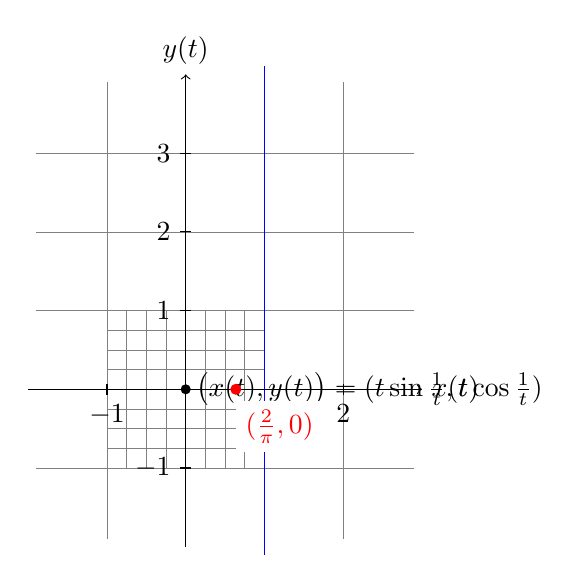
\begin{tikzpicture}
  \draw[gray,very thin] (-1.9,-1.9) grid (2.9,3.9)
          [step=0.25cm] (-1,-1) grid (1,1);
  \draw[blue] (1,-2.1) -- (1,4.1); % asymptote

  \draw[->] (-2,0) -- (3,0) node[right] {$x(t)$};
  \draw[->] (0,-2) -- (0,4) node[above] {$y(t)$};

  \foreach \pos in {-1,2}
    \draw[shift={(\pos,0)}] (0pt,2pt) -- (0pt,-2pt) node[below] {$\pos$};

  \foreach \pos in {-1,1,2,3}
    \draw[shift={(0,\pos)}] (2pt,0pt) -- (-2pt,0pt) node[left] {$\pos$};

  \fill (0,0) circle (0.064cm);
  \draw[thick,parametric,domain=0.4:1.5,samples=200]
    % The plot is reparameterised such that there are more samples
    % near the center.
    plot[id=asymptotic-example] function{(t*t*t)*sin(1/(t*t*t)),(t*t*t)*cos(1/(t*t*t))}
    node[right] {$\bigl(x(t),y(t)\bigr) = (t\sin \frac{1}{t}, t\cos \frac{1}{t})$};

  \fill[red] (0.63662,0) circle (2pt)
    node [below right,fill=white,yshift=-4pt] {$(\frac{2}{\pi},0)$};
\end{tikzpicture}
\end{codeexample}

\include{parts/The-Basic-Layer/sections/pgfmanual-en-base-design}
\include{parts/The-Basic-Layer/sections/pgfmanual-en-base-scopes}
\include{parts/The-Basic-Layer/sections/pgfmanual-en-base-points}
\include{parts/The-Basic-Layer/sections/pgfmanual-en-base-paths}
\include{parts/The-Basic-Layer/sections/pgfmanual-en-base-decorations}
\include{parts/The-Basic-Layer/sections/pgfmanual-en-base-actions}
\include{parts/The-Basic-Layer/sections/pgfmanual-en-base-arrows}
\include{parts/The-Basic-Layer/sections/pgfmanual-en-base-nodes}
\include{parts/The-Basic-Layer/sections/pgfmanual-en-base-matrices}
\include{parts/The-Basic-Layer/sections/pgfmanual-en-base-transformations}
\include{parts/The-Basic-Layer/sections/pgfmanual-en-base-patterns}
\include{parts/The-Basic-Layer/sections/pgfmanual-en-base-images}
\include{parts/The-Basic-Layer/sections/pgfmanual-en-base-external}
\include{parts/The-Basic-Layer/sections/pgfmanual-en-base-plots}
\include{parts/The-Basic-Layer/sections/pgfmanual-en-base-layers}
\include{parts/The-Basic-Layer/sections/pgfmanual-en-base-shadings}
\include{parts/The-Basic-Layer/sections/pgfmanual-en-base-transparency}
\include{parts/The-Basic-Layer/sections/pgfmanual-en-base-animations}
\include{parts/The-Basic-Layer/sections/pgfmanual-en-base-internalregisters}
\include{parts/The-Basic-Layer/sections/pgfmanual-en-base-quick}
% \input{parts/The-System-Layer/The-System-Layer.tex}
% \input{parts/References-and-Index/References-and-Index.tex}
    
\end{document}